\documentclass[10pt,a4paper]{article}
\usepackage[margin=17mm,headheight=14pt,footskip=10mm]{geometry}
\usepackage{fontspec,unicode-math}
\setmainfont{Latin Modern Roman}
\setsansfont{Latin Modern Sans}
\setmathfont{Latin Modern Math}
\usepackage{amsmath,graphicx,booktabs,array,tabularx,xcolor,colortbl,fancyhdr,enumitem}
\usepackage[most]{tcolorbox}
\usepackage[hidelinks]{hyperref}
\definecolor{ink}{HTML}{123D54}
\definecolor{pale}{HTML}{EFF4F6}
\pagestyle{fancy}\fancyhf{}
\fancyfoot[L]{\sffamily\scriptsize APD background / interference — discussion draft — 6 October 2026}
\fancyfoot[R]{\sffamily\scriptsize\thepage}
\renewcommand{\headrulewidth}{0pt}
\emergencystretch=3em
\setlength{\parindent}{0pt}\setlength{\parskip}{6pt}
\setlength{\abovedisplayskip}{7pt}\setlength{\belowdisplayskip}{7pt}
\renewcommand{\arraystretch}{1.18}
\newcolumntype{Y}{>{\raggedright\arraybackslash}X}
\newcommand{\heading}[1]{{\sffamily\Large\bfseries\color{ink}#1}\par\vspace{7pt}}
\newtcolorbox{fitbox}[1]{colback=pale,colframe=ink,boxrule=0.35pt,arc=0pt,left=6pt,right=6pt,top=4pt,bottom=4pt,title=#1,fonttitle=\sffamily\bfseries\small,fontupper=\small}
\begin{document}

\heading{APD background and interference\newline Fit comparison for discussion with Richard}
Revised 6 October 2026 • Daping / Richard • Analysis of the supplied 40 s APD recording. This is a comparison of saved fits and sensitivity tests, not a calibration of absolute orientation. No new optimization was performed to prepare this report.\par
\textbf{Main result.} The inferred background and polar-angle range depend strongly on the allowed field. The earlier \textasciitilde{}55\% background solution is not uniquely required: a broader stationary-field model reaches similar agreement at 20–30\%, and the tested axial-motion model reaches similar agreement at 10\%. These explanations cannot yet be distinguished with this recording alone.\par
\textbf{What to discuss first.} Figures 1–2 show what the models actually fit; Figure 3 compares background makeup and angle ranges; Figure 5 shows how large background can coexist with the measured intensity through signed interference. The rest records the assumptions, controls and limits.\par
{\footnotesize\setlength{\tabcolsep}{4pt}\begin{tabularx}{\linewidth}{>{\hsize=1.598\hsize}Y>{\hsize=0.845\hsize}Y>{\hsize=1.113\hsize}Y>{\hsize=0.722\hsize}Y>{\hsize=0.722\hsize}Y}\toprule\rowcolor{pale}
\textbf{Model} & \textbf{BG / Tmax (\%)\newline 30 s / 10 s} & \textbf{Held-out XY RMS\newline 30 s / 10 s} & \textbf{\(θ\) range (\textdegree{})\newline 30–31 s} & \textbf{\(θ\) range (\textdegree{})\newline 10–11 s}\\\midrule
BG only & 31.7 / 34.6 & 0.0896 / 0.0989 & 37.3–89.2 & 42.0–90.0\\
Additive + sqrt extension & 38.5 / 39.9 & 0.0927 / 0.1024 & 34.6–89.9 & 39.0–89.7\\
5-mode shared, relaxed & 54.7 / 54.4 & 0.0281 / 0.0460 & 12.5–89.7 & 17.8–89.7\\
General stationary, \(\leq\)30\% & 30.0 / 29.8 & 0.0288 / 0.0387 & 30.9–64.8 & 32.7–63.3\\
General stationary, relaxed & 55.0 / 54.7 & 0.0245 / 0.0408 & 6.4–89.7 & 11.6–89.8\\
Axial R\(\leq\)300 nm, \(\leq\)10\% & 10.0 / 9.9 & 0.0308 / 0.0411 & 34.6–55.2 & 37.2–53.7\\
\bottomrule\end{tabularx}}\par\medskip
Direct inversion without background gives \(θ\)=27.4–57.7\textdegree{} at 30–31 s and 26.9–57.0\textdegree{} at 10–11 s. These are descriptive baselines, not known angles. All \(θ\) ranges are folded to 0–90\textdegree{} and sampled at the 128 fitted bins; none is a confidence interval.\par
\textbf{Three conclusions supported by these calculations:} (i) simply changing the measured hole outline has very little effect in the tested pupil-mask model; (ii) the restricted hole-edge field tested here is insufficient; (iii) stationary-field structure and source position can trade against background power and recovered angles. A good cone fit alone cannot resolve that tradeoff.\par
\textbf{Stopping point.} Retain NA\textsubscript{in}=0.38 and the current correction matrix. Do not choose a final background subtraction or publish absolute \(θ\) from the best residual alone. Decide which physical constraint or perturbation is worth measuring next.\par
\clearpage
\heading{1. What the plotted averages mean}
The plots compare repeated traversals of the same measured anisotropy trajectory, taken from two windows of the 40 s APD recording. Each traversal retains its acquisition order, including the two branches. Channel intensities are averaged first; X and Y are calculated afterwards.\par
{\footnotesize\setlength{\tabcolsep}{4pt}\begin{tabularx}{\linewidth}{>{\hsize=0.649\hsize}Y>{\hsize=1.423\hsize}Y>{\hsize=0.928\hsize}Y}\toprule\rowcolor{pale}
\textbf{Plot label} & \textbf{What it contains} & \textbf{How it is used}\\\midrule
Training average & One alternating set of complete traversals: cycles 1,3,5,… & The model parameters are chosen using this average.\\
Held-out average & The other set: cycles 2,4,6,… & The fitted prediction is compared with this average without refitting.\\
Fitted prediction & The four-channel forward model evaluated along its fitted cone & The same prediction is shown against both averages.\\
\bottomrule\end{tabularx}}\par\medskip
{\footnotesize\setlength{\tabcolsep}{4pt}\begin{tabularx}{\linewidth}{>{\hsize=1.021\hsize}Y>{\hsize=0.990\hsize}Y>{\hsize=0.990\hsize}Y}\toprule\rowcolor{pale}
\textbf{Window} & \textbf{Training traversals} & \textbf{Held-out traversals}\\\midrule
30–31 s & 152 & 152\\
10–11 s & 109 & 108\\
\bottomrule\end{tabularx}}\par\medskip
Both averages estimate the same trajectory within the same second. Agreement between them shows how reproducible the averaged curve is. A prediction that agrees with both is less likely to be following fluctuations peculiar to just one set. However, both sets share calibration, processing and any persistent distortion: this does not establish correct background or correct angles, and is not prediction of a new recording.\par
The broad two-pass shape repeats; the 10–11 s window is more internally consistent than 30–31 s. All anisotropy axes remain \(-\)1 to +1. The plotted convention is:\par
\begin{equation*}X=\frac{I_0-I_{90}}{I_0+I_{90}},\qquad Y=\frac{I_{45}-I_{135}}{I_{45}+I_{135}}\end{equation*}
Fixed optical baseline: current gains and inverse T matrix, NA 0.38–1.30, water/oil indices 1.33/1.51, corrected Fresnel and BFP mapping. Detailed preprocessing and optimization records remain in the accompanying scripts; they are not needed to read these plots.\par
\clearpage
\heading{2A. Common signal and power notation}
Here T means the sum of all four corrected channel intensities. S is rod-only intensity, B is background-only intensity, and C is the signed interference contribution. For every family:\par
\begin{equation*}I_j(\chi)=S_j(\chi)+C_j(\chi)+B_j\end{equation*}
\begin{equation*}T(\chi)=\sum_j I_j(\chi)=S(\chi)+C(\chi)+B\end{equation*}
The instantaneous unit rod direction is d=(sin\(θ\) cos\(φ\), sin\(θ\) sin\(φ\), cos\(θ\)), and \(χ\) labels position around the cone. In field equations \(θ\) describes that direction over 0–180\textdegree{}; the reported angle plots fold it to 0–90\textdegree{}. This distinction preserves the sign of \(d_{z}\) when evaluating interference.\par
\begin{equation*}E_{s,j}(u,\chi)=a_0(d_x+i d_y)\sum_{l=x,y,z}d_l F_{jl}(u)\end{equation*}
F is the fixed collected dipole field, including the optics. The one constant a\textsubscript{0} per interval sets the overall rod brightness. The factor \(d_{x}\)+i \(d_{y}\)=sin\(θ\) exp(i\(φ\)) supplies the circular-excitation amplitude AND phase. It is not a freely chosen brightness at each point.\par
\begin{equation*}S_j=a_0^2\sin^2\theta\,q_j(\theta,\phi)\end{equation*}
\begin{equation*}q_j=A_F+B_F\sin^2\theta+C_F\sin^2\theta\cos[2(\phi-\psi_j)]\end{equation*}
\begin{equation*}S(\theta)=4a_0^2\sin^2\theta\,(A_F+B_F\sin^2\theta)\end{equation*}
For the annulus, \(ψ\)\_j=0\textdegree{},90\textdegree{},45\textdegree{},135\textdegree{}; \(A_{F}\)=0.89080598, \(B_{F}\)=0.10919402, \(C_{F}\)=0.92778057. The F subscripts distinguish the optical coefficients from background B and interference C. The shared-field code evaluates the corresponding pupil integrals numerically. Individual signal channels vary with \(θ\) and \(φ\); their ideal annular sum varies with \(θ\) only.\par
\textbf{Constant versus varying:} a\textsubscript{0} and the optical response are constant within an interval. \(θ\) and \(φ\) vary along the cone. In all stationary-background families below, \(B_{j}\) and their sum B are constant; it is \(C_{j}\) and C that may change with orientation. A negative C reduces measured power without making S or B negative.\par
\begin{fitbox}{Common to the physical cone fits}Per interval: motor-axis tilt and azimuth, cone half-angle (3); starting mechanical phase and monotone phase increments (16); one constant brightness scale a\textsubscript{0} (1). Total: 20 local real parameters per interval. Counts describe the parameterization, not a guarantee that every parameter is identifiable. Optical coefficients, NA, Fresnel/BFP response and the current gains/matrix are held fixed.\end{fitbox}
\clearpage
\heading{2B. Additive backgrounds: notebook versus Stokes}
\textbf{The original notebook was less restrictive.} It fitted three background parameters, not four independent channel offsets:\par
\begin{equation*}(B_0,B_{90},B_{45},B_{135})=\frac{d_c}{2}(1+f_a,1-f_a,1+f_b,1-f_b)\end{equation*}
\begin{equation*}d_c\geq0,\qquad -1\leq f_a\leq1,\qquad -1\leq f_b\leq1\end{equation*}
This guarantees nonnegative channel backgrounds and equal pair sums. The current Stokes version has the same algebra after the following substitution, but restricts the allowed region from a square to its inscribed disk:\par
\begin{equation*}B=2d_c,\quad f_a=p\cos(2\alpha),\quad f_b=p\sin(2\alpha),\quad f_a^2+f_b^2\leq1\end{equation*}
For example, \(f_{a}\)=\(f_{b}\)=1 is allowed by the notebook but excluded by a common physical Stokes background. Thus the two models agree inside the disk, but are not equivalent over their full allowed parameter ranges. Four fully independent offsets would be more general still because they need not have equal pair sums.\par
\textbf{1. Background only.} There is no modeled interference. Each channel has a constant additive intensity:\par
\begin{equation*}I_j=S_j+B_j,\qquad C_j=0\end{equation*}
\begin{equation*}T=4a_0^2\sin^2\theta(A_F+B_F\sin^2\theta)+B\end{equation*}
The background is represented by a positive Stokes intensity pattern. This allows a constant polarization imbalance without making any channel negative:\par
\begin{equation*}B_j=\frac{B}{4}\{1+p\cos[2(\psi_j-\alpha)]\},\qquad 0\leq p\leq1\end{equation*}
\clearpage
\heading{2B (continued). Meaning of the Stokes restriction}
This is a \textbf{common-background assumption}, not a universal law for all offsets. One optical background observed through ideal linear analyzers has Stokes parameters S\textsubscript{0},S\textsubscript{1},S\textsubscript{2} with nonnegative coherence matrix. Setting B=2S\textsubscript{0} gives:\par
\begin{equation*}B_j=\frac12\left[S_0+S_1\cos(2\psi_j)+S_2\sin(2\psi_j)\right]\end{equation*}
\begin{equation*}p=\frac{\sqrt{S_1^2+S_2^2}}{S_0}\leq1,\qquad B_0+B_{90}=B_{45}+B_{135}=B/2\end{equation*}
B, p and \(α\) are constant. This permits polarized or unpolarized background while enforcing physical channel intensities and equal pair sums. “Positive” refers to the physical intensity/coherence matrix, not to requiring S\textsubscript{1} and S\textsubscript{2} individually to be positive. Circular Stokes S\textsubscript{3} is not measured by these linear analyzers. Electronic offsets, unequal detector acceptance, calibration errors or independent post-analyzer backgrounds need not satisfy this pattern; four independent nonnegative offsets would be a different model.\par
\begin{fitbox}{Background only: fitted quantities}B, p, \(α\) (3 background parameters), plus the 20 local cone/phase/brightness parameters: 23 per interval. C=0. Fits are separate in the two windows.\end{fitbox}
The original solver fitted cone geometry (3) plus \(d_{c}\),\(f_{a}\),\(f_{b}\) (3) against anisotropy shape. The current comparison also constrains ordered channels and total power with one a\textsubscript{0} per interval. Consequently its residual/angle differences cannot be attributed solely to the disk constraint. Saved legacy square-versus-disk controls exist, but no new controlled refit was run for this revision.\par
\clearpage
\heading{2C. Richard’s four-coefficient approximation}
The quoted email proposes a correction whose value changes with the real signal, but whose coefficient is constant within each channel:\par
\begin{equation*}I_{m,j}=I_{r,j}+D_j(I_{r,j}),\qquad D_j(I_{r,j})=C_j\sqrt{I_{r,j}}\end{equation*}
\begin{equation*}T(\theta,\phi)=S(\theta)+\sum_j C_j\sqrt{S_j(\theta,\phi)}\end{equation*}
\begin{fitbox}{What Richard’s quoted model fits}Four real coefficients \(C_{j}\), one per channel. With our common fixed-excitation cone framework this would mean 4 correction parameters plus 20 local parameters = 24 per separately fitted interval. This exact four-coefficient model has NOT been run in the saved comparison.\end{fitbox}
The \(C_{j}\) can have either sign. They are constants in this approximation; \(D_{j}\) varies because the signal varies. Phase is not absent: phase and spatial overlap are absorbed into each \(C_{j}\). For a fixed, perfectly matched single-mode background field of amplitude \(b_{j}\), the full optical intensity is:\par
\begin{equation*}I_{m,j}=I_{r,j}+|b_j|^2+2|b_j|\cos\delta_j\sqrt{I_{r,j}}\end{equation*}
\begin{equation*}C_j=2|b_j|\cos\delta_j\quad\hbox{(matched single mode)}\end{equation*}
Writing C=2 cos(phase) requires the background amplitude to have been normalized to one or absorbed into the intensity units. Otherwise C has units of square-root intensity. With spatially integrated fields, the effective coefficient includes overlap and need not stay constant as rod orientation changes.\par
The quoted equation omits the background-only intensity |\(b_{j}\)|\textsuperscript{2}. It therefore describes an approximation where that term is neglected, or a signal from which it has already been removed. It is not obtained by setting the background power to zero in a full coherent model: that would also remove the cross term.\par
For positive measured intensity, the nonnegative-amplitude solution is:\par
\begin{equation*}I_{r,j}=\left[\frac{-C_j+\sqrt{C_j^2+4I_{m,j}}}{2}\right]^2\end{equation*}
The email’s suggested x,y,S\textsubscript{1},S\textsubscript{2} notation is a possible way to express four quantities; without its precise definitions it should not be equated with the three-parameter physical Stokes background used in 2B. The direct \(C_{j}\) representation avoids that ambiguity.\par
\clearpage
\heading{2C (continued). The extension actually fitted}
The plots previously labeled “Richard effective” are from a different, seven-parameter background/interference model:\par
\begin{equation*}I_{m,j}=S_j+B_j+2c_j\sqrt{B_jS_j},\qquad |c_j|\leq1\end{equation*}
\begin{equation*}T=S+B+2\sum_j c_j\sqrt{B_jS_j}\end{equation*}
\begin{equation*}C_j^{\mathrm{eff}}=2c_j\sqrt{B_j},\qquad |C_j^{\mathrm{eff}}|\leq2\sqrt{B_j}\end{equation*}
\begin{fitbox}{Fitted quantities in the saved extension}Three constant Stokes-background parameters B,p,\(α\) plus four constant real overlap coefficients \(c_{j}\): 7, or 27 including the local cone/phase/brightness parameters, per interval. Coefficients and backgrounds were fitted separately in the two windows.\end{fitbox}
This is additive background plus an effective interference term. Relative phase and spatial overlap are folded into \(c_{j}\) rather than fitted separately. At a fixed \(c_{j}\) its interference magnitude follows \(\surd\)\(S_{j}\), and its channelwise sign is fixed; the total signed cross term may still change sign as channels vary.\par
The added \(B_{j}\) term and its bound on \(C_{j}\) distinguish this extension from Richard’s quoted approximation. The extension reduces to the quoted mathematical form only after its additive \(B_{j}\) is removed from the measured intensity, with the remaining coefficient identified as \(C_{j}\)=2c\_j\(\surd\)\(B_{j}\). That identification still retains constraints absent from a free four-C fit.\par
Neither four independent \(c_{j}\) nor the bound alone proves that one stationary vector field can realize them throughout a trajectory. In a coherent field model, the overlap may depend on orientation; treating it as constant is the approximation being tested.\par
All displayed fit scores, fitted background powers and angle ranges under the revised label “Additive + sqrt extension” refer to this saved seven-parameter model. They cannot be used to claim that Richard’s exact four-coefficient proposal has succeeded or failed. No new fits were run for this editorial correction.\par
\clearpage
\heading{2D. Uniform field and uniform-plus-radial field}
\textbf{3. Uniform transverse background.} Let \(b_{x}\) and \(b_{y}\) be constant complex field amplitudes in normalized uniform pupil modes. Let U be the total extra noninterfering background. Then:\par
\begin{equation*}T=S(\theta)+2(|b_x|^2+|b_y|^2)+U+C_{\mathrm{uni}}(\theta,\phi)\end{equation*}
\begin{equation*}C_{\mathrm{uni}}=4a_0\Gamma\sin^2\theta\,\mathrm{Re}\{e^{i\phi}(b_x^*\cos\phi+b_y^*\sin\phi)\}\end{equation*}
\(Γ\) is the fixed overlap between the collected transverse dipole field and a normalized uniform pupil field, computed from the annulus/Fresnel/BFP optics. It is not an extra adjustable overlap at each point. Both complex b coefficients and U are constant. The cross term changes magnitude and can change sign through \(θ\) and \(φ\), even though the background field itself stays fixed.\par
\begin{fitbox}{Uniform field: fitted quantities}Two complex amplitudes \(b_{x}\),\(b_{y}\) (4 real values) and noninterfering Stokes parameters U,\(p_{U}\),\(α\)\_U (3): 7 background parameters, or 27 including local parameters, per interval. \(Γ\) is fixed by the optics.\end{fitbox}
\textbf{4. Uniform plus radial background.} Add the normalized collected field pattern of a z-directed dipole, with constant complex amplitude \(b_{r}\):\par
\begin{equation*}T=S(\theta)+2(|b_x|^2+|b_y|^2+|b_r|^2)+U+C_{\mathrm{uni}}+C_{\mathrm{rad}}\end{equation*}
\begin{equation*}C_{\mathrm{rad}}=8a_0\kappa\sin\theta\cos\theta\,\mathrm{Re}(e^{i\phi}b_r^*),\qquad \kappa=\sqrt{A_F/2}\end{equation*}
The radial mode adds a different orientation dependence: sin\(θ\) cos\(θ\) times a \(φ\)-dependent phase projection. Its intensity is still constant. In these normalized, mutually orthogonal pupil modes, summed coherent background power is twice the sum of squared field amplitudes. Cross terms between background modes need not vanish in every individual analyzer channel; they are retained in the channel calculation.\par
U is distributed across channels by the same positive Stokes form as above. “Noninterfering” means no cross term with the modeled rod signal: it can include incoherent light or a coherent field with no relevant spatial overlap. These expressions describe a background family, not a claim that a uniform or radial pattern came from a particular optical surface.\par
The separate-interval three-mode fits allow their field coefficients to change between windows. The shared three-mode test fixes the same coefficients and U across both windows, while each window retains its own cone and a\textsubscript{0}. A budget cap changes the allowed power, not these equations.\par
\begin{fitbox}{Uniform + radial: fitted quantities}Add complex \(b_{r}\) (2 real values): 9 background parameters. Separate fits have 29 parameters per interval; the shared three-mode fit has 9 shared plus 20 local per window, totaling 49. \(κ\) is fixed by \(A_{F}\).\end{fitbox}
\clearpage
\heading{2E. Five modes, general stationary field and hole edge}
These families have the same power equation. They differ in which fixed spatial/polarization patterns \(g_{m}\) are available to form the background:\par
\begin{equation*}E_{b,j}(u)=\sum_{m=1}^{M}b_m g_{jm}(u)\end{equation*}
\begin{equation*}H^{\Sigma}_{lm}=\sum_j\int F_{jl}(u)g_{jm}^*(u)\,du\end{equation*}
\begin{equation*}T=S(\theta)+2\sum_{m=1}^{M}|b_m|^2+U+C_M(\theta,\phi)\end{equation*}
\begin{equation*}C_M=2a_0\,\mathrm{Re}\!\left[(d_x+i d_y)\sum_{l,m}d_l H^{\Sigma}_{lm}b_m^*\right]\end{equation*}
The modes are orthonormal before analyzer projection, giving the factor 2 in total background power for this four-analyzer convention. H is a precomputed optical overlap, constant for a stationary source. The \(b_{m}\) and U are constant. Thus orientation changes \(C_{M}\) through the displayed products of direction components; no per-point overlap is fitted.\par
{\footnotesize\setlength{\tabcolsep}{4pt}\begin{tabularx}{\linewidth}{>{\hsize=0.619\hsize}Y>{\hsize=1.639\hsize}Y>{\hsize=0.742\hsize}Y}\toprule\rowcolor{pale}
\textbf{Family} & \textbf{Allowed background pattern} & \textbf{Final total-intensity form}\\\midrule
5-mode shared & Uniform x/y plus orthogonalized collected z-, x- and y-dipole patterns & T=S + 2\(Σ\)\textsubscript{1}\textsuperscript{5}|b\textsubscript{m}|\textsuperscript{2} + U + C\textsubscript{5}\\
General stationary & Each transverse polarization uses the five-dimensional scalar span of the collected dipole components (10 modes) & T=S + 2\(Σ\)\textsubscript{1}\textsuperscript{10}|b\textsubscript{m}|\textsuperscript{2} + U + C\textsubscript{10}\\
Hole-edge surrogate & Two transverse polarizations \(\times\) three edge-localized angular patterns (6 modes) & T=S + 2\(Σ\)\textsubscript{1}\textsuperscript{6}|b\textsubscript{m}|\textsuperscript{2} + C\textsubscript{6}; U=0\\
\bottomrule\end{tabularx}}\par\medskip
The edge patterns use exp[\(-\)(\(ρ\)\(-\)0.38)\textsuperscript{2}/(2w\textsuperscript{2})] times 1, cos\(ϕ\)\_u or sin\(ϕ\)\_u, then normalization/orthogonalization. Here \(ϕ\)\_u is pupil azimuth, not rod azimuth \(φ\). Width w is fixed for each tested case. The six complex amplitudes are shared across both windows, as are the five-/ten-mode coefficients in the corresponding shared fits.\par
For a stationary field, \(C_{M}\) is quadratic in d and has mechanical-phase harmonics only up to order two on the cone; S is quartic and can reach order four. Increasing the mode family changes the allowed quadratic coefficients, not the permission to choose an arbitrary C at every bin. The ten-mode completeness statement assumes a fixed-position ideal dipole, common pupil and full collection.\par
\begin{fitbox}{Fitted quantities for each stationary family}Five-mode: 5 complex \(b_{m}\) plus U,\(p_{U}\),\(α\)\_U = 13 shared background parameters; 53 including both windows. General stationary: 10 complex \(b_{m}\) plus U,\(p_{U}\),\(α\)\_U = 23 shared; 63 total. Edge: 6 complex \(b_{m}\) = 12 shared; 52 total, with U fixed to zero. Mode shapes, overlaps and edge width w are fixed for each case; background caps are imposed limits, not fitted parameters.\end{fitbox}
\clearpage
\heading{2F. Axial motion, mask and deliberately flexible controls}
\textbf{5. Bounded axial motion with a stationary background.} The ten background coefficients stay fixed. The rod position changes its phase relative to that field, so the optical overlap now depends on z:\par
\begin{equation*}z(\chi)=R\sin\theta_{\mathrm{axis}}\cos(\chi+\delta),\quad f(z)=[1+(z/z_R)^2]^{-1/2}\end{equation*}
\begin{equation*}H^{\Sigma}_{lm}(z)=\sum_j\int F_{jl}g_{jm}^*e^{ikz[n_w+\sqrt{n_w^2-\rho^2}]}\,du\end{equation*}
\begin{equation*}T=f(z)^2S(\theta)+2\sum_{m=1}^{10}|b_m|^2+U+C_{10}(\theta,\phi,z)\end{equation*}
\begin{equation*}C_{10}=2a_0 f(z)\,\mathrm{Re}\!\left[e^{-i\arctan(z/z_R)}(d_x+i d_y)\sum_{l,m}d_l H^{\Sigma}_{lm}(z)b_m^*\right]\end{equation*}
R and \(δ\) are constants per interval; \(z_{R}\)=2 \(\mu\)m and k=2\(π\)/(633 nm) are fixed in these tests. Background intensity is still constant. \(θ\), \(φ\) and z vary together along the trajectory. The signal acquires f\textsuperscript{2}; interference acquires f and a deterministically changing propagation/Gouy phase. There is no independent focus multiplier per point. The separate finite-aperture simulation changes collection itself and was not included in this fitted power equation.\par
\begin{fitbox}{Axial motion: fitted quantities}The general field’s 23 shared background parameters, 20 local parameters per window, and R,\(δ\) per window: 67 total. Radius cap, wavelength and \(z_{R}\) are fixed scenario settings.\end{fitbox}
\clearpage
\heading{2F (continued). Mask and flexible controls}
\textbf{Measured-mask variant.} The mask changes the fixed signal response and overlaps, not the basic power balance:\par
\begin{equation*}T=a_0^2|d_x+i d_y|^2\,\mathbf{d}^{T}Q^{\Sigma}_{\mathrm{mask}}\mathbf{d}+C_{\mathrm{mask}}(\mathbf{d})+B\end{equation*}
Q and H are recomputed through the measured aperture, and B remains constant. The asymmetric mask may introduce \(φ\) dependence even into rod-only total power. The mask fits used the three-mode background family; an amplitude mask does not model light scattered from the hole wall.\par
\begin{fitbox}{Measured mask: fitted quantities}The same three complex field amplitudes and noninterfering Stokes background as the separate three-mode fits: 29 parameters per window. Mask geometry/rotation and the resulting Q,H are fixed in each comparison.\end{fitbox}
\textbf{Arbitrary-overlap feasibility control, not a stationary-field fit:}\par
\begin{equation*}T=S+B+2\sum_j\rho_j(\chi)\sqrt{S_j(\chi)B_j},\qquad |\rho_j(\chi)|\leq1\end{equation*}
Here \(B_{j}\) stay constant but every \(ρ\)\_j can vary independently at every point. That freedom can reproduce the data exactly without demonstrating one realizable stationary field. The earlier free-brightness models additionally replaced the prescribed a\textsubscript{0} sin\(θ\) by an independently recovered amplitude a(\(χ\)):\par
\begin{equation*}T=a(\chi)^2Q(\theta,\phi)+a(\chi)L(\theta,\phi)+B\end{equation*}
Q is the summed collection response for unit excitation amplitude; L is the cross-term coefficient for the selected background family. These are historical relaxations, not the main fixed-excitation results.\par
\begin{fitbox}{Flexible controls: what is adjustable}Free-overlap test: cone, phase and a\textsubscript{0} determine S; constant \(B_{j}\) are selected under scalar feasibility bounds (the 10\% witness fixes equal \(B_{j}\)). Each \(ρ\)\_j(\(χ\)) is then constructed point by point to match \(I_{j}\), rather than predicted by one field. Earlier free-brightness fits similarly recover a(\(χ\)) from the measured total at every bin; this adds pointwise freedom even though those amplitudes are not independent optimizer coordinates.\end{fitbox}
\clearpage
\heading{3. What the older model families can reproduce}
\begin{center}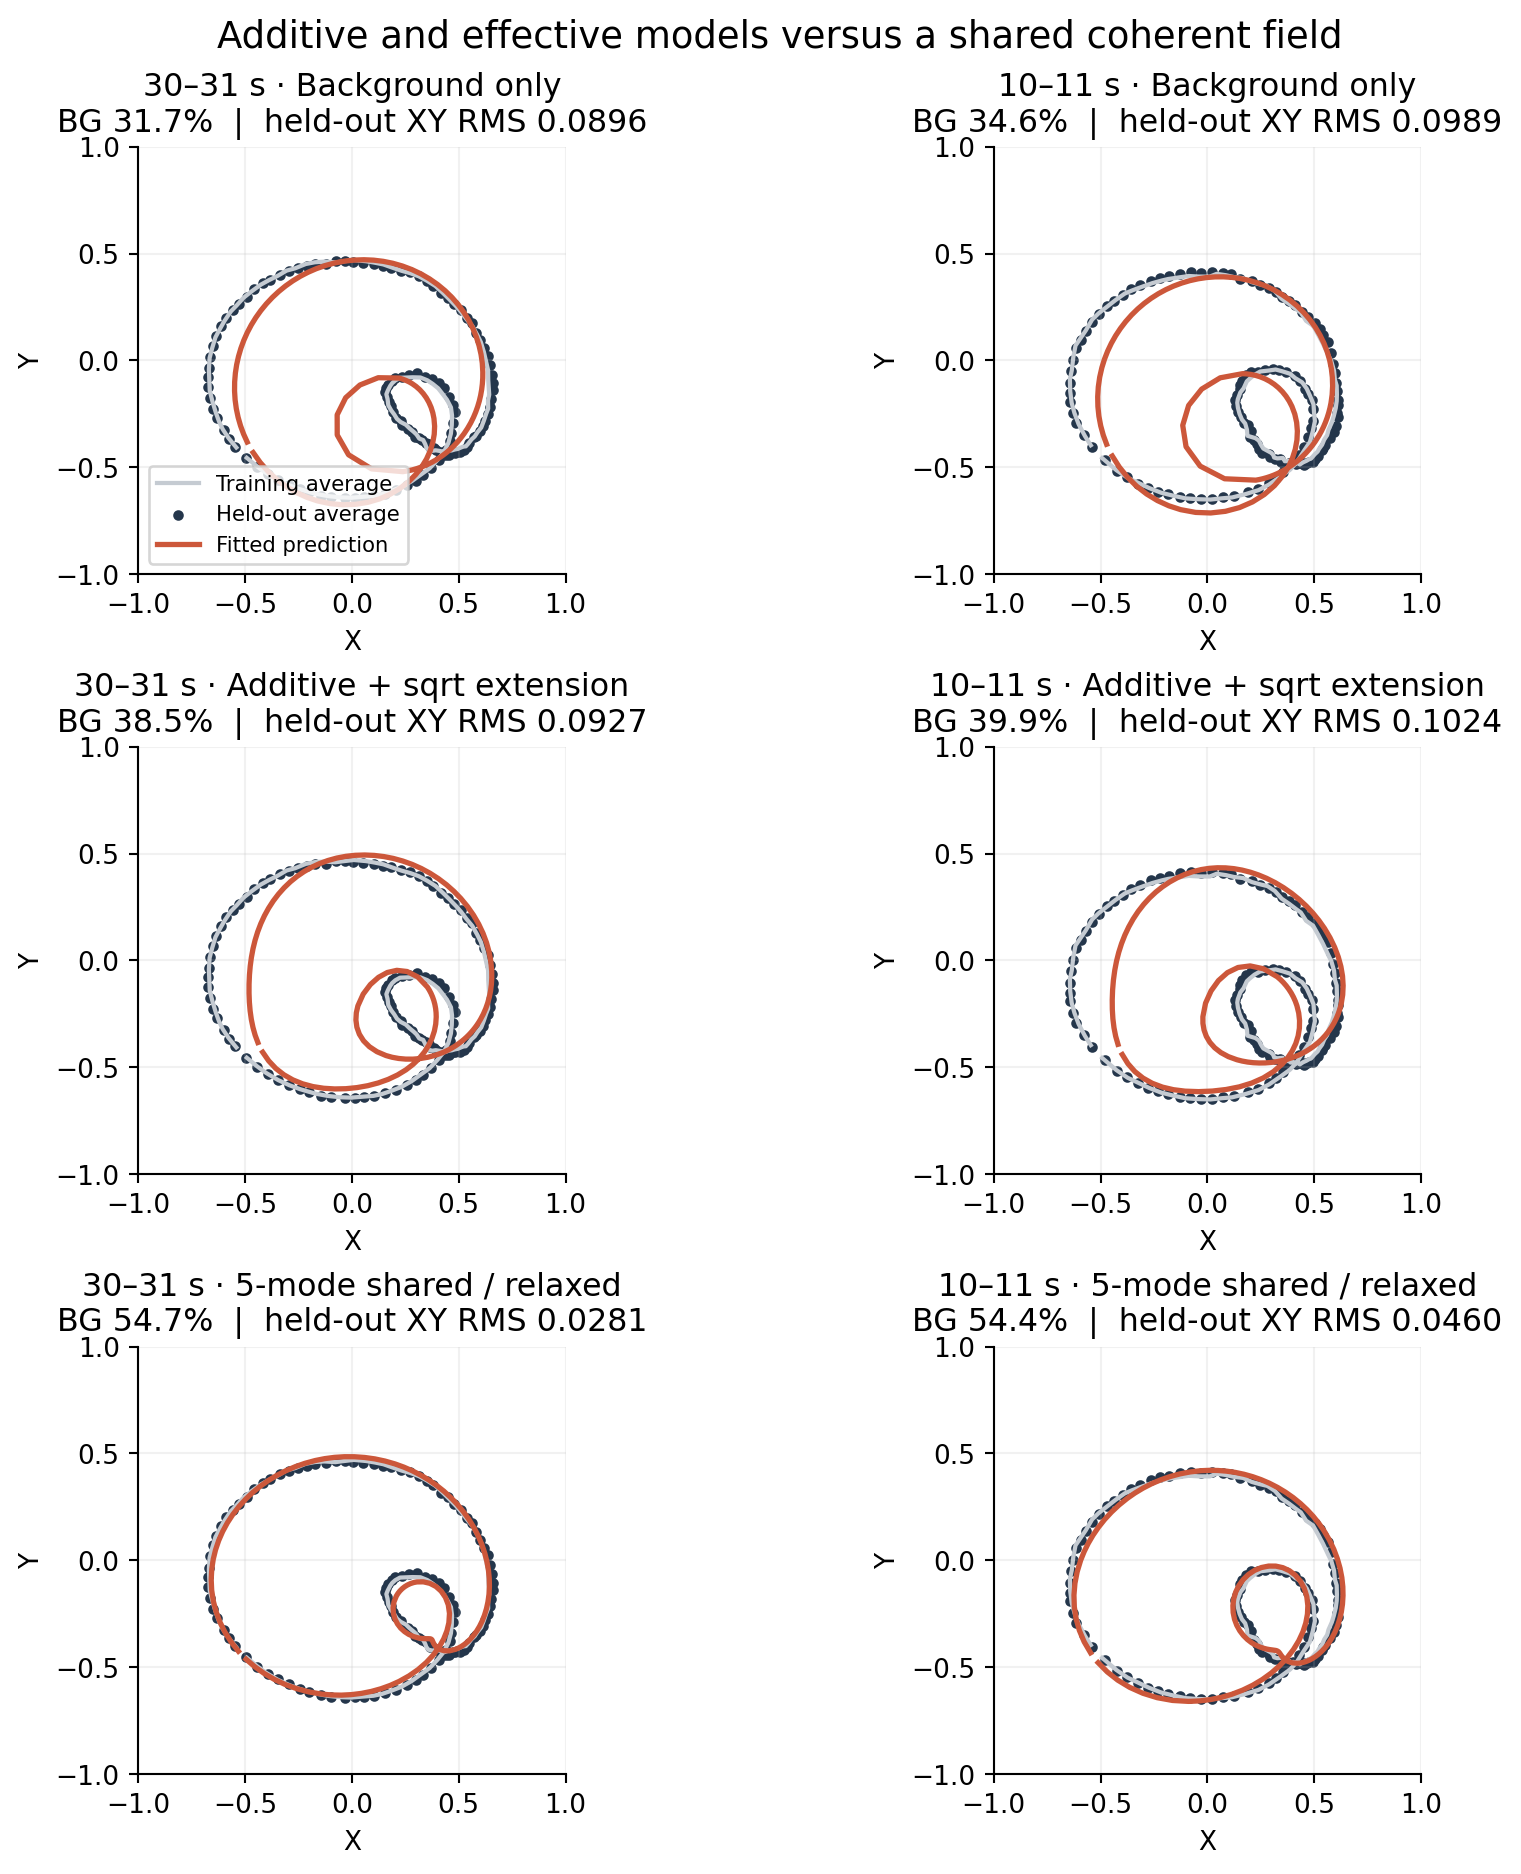
\includegraphics[width=\linewidth,height=7.15in,keepaspectratio]{figures/01_model_fits.png}\end{center}
Figure 1. Points are held-out cycle averages; grey is the training average; red is the saved prediction. The additive and additive-plus-sqrt fits are separate per interval. The five-mode field uses the same absolute background coefficients in both intervals. All three use constant a\textsubscript{0} with circular-excitation dependence. The additive-plus-sqrt extension need not win on XY RMS because that is not the channel fitting objective.\par
\clearpage
\heading{4. Comparable fits with smaller background budgets}
\begin{center}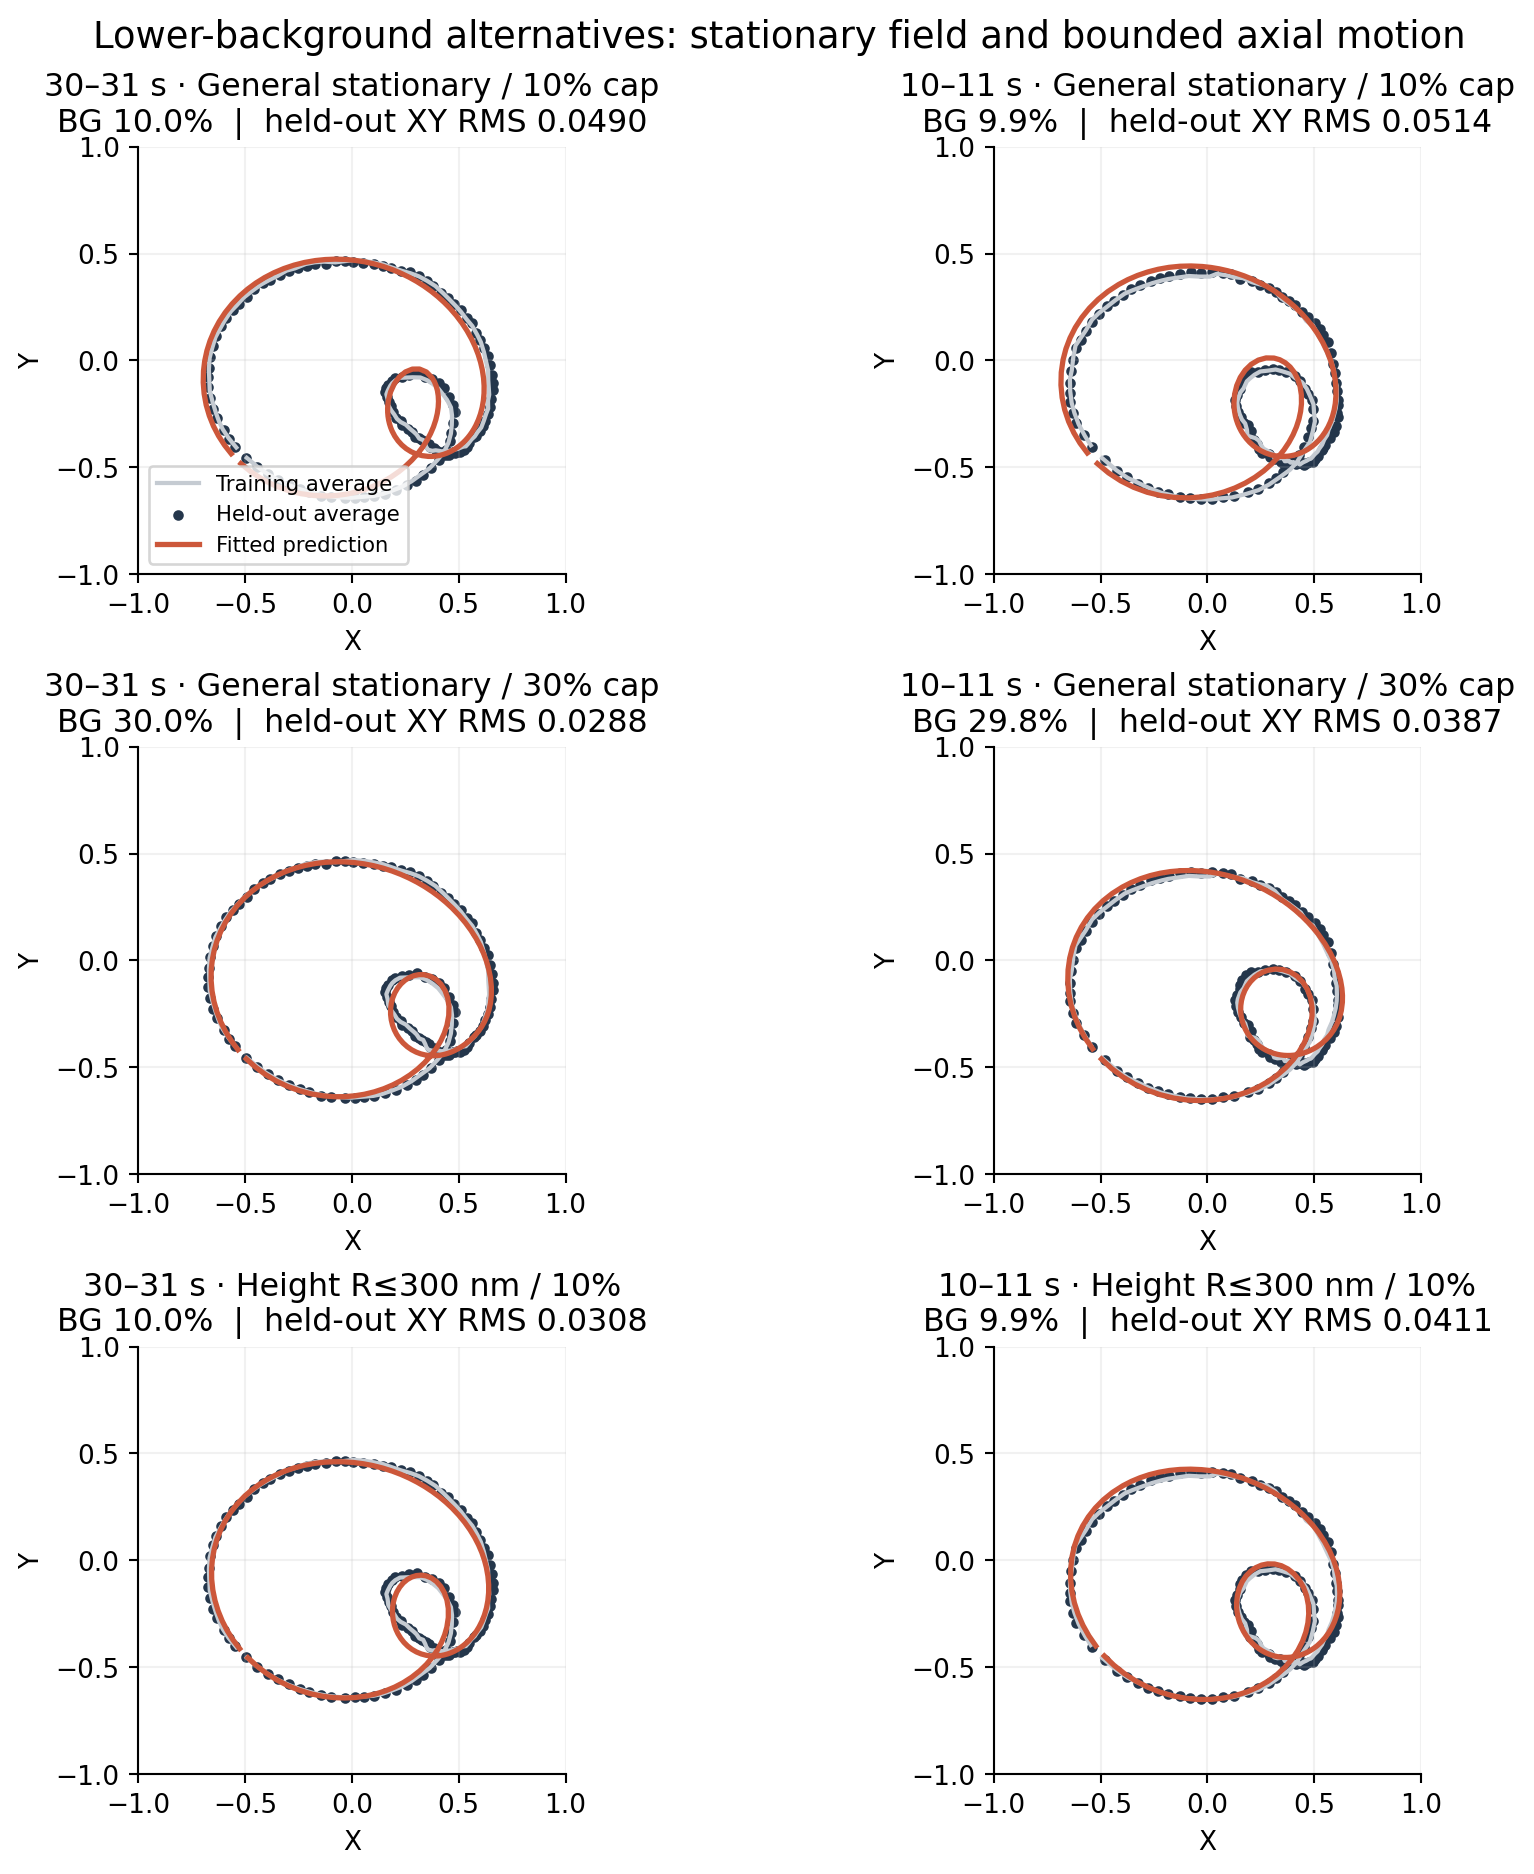
\includegraphics[width=\linewidth,height=7.15in,keepaspectratio]{figures/02_low_background_fits.png}\end{center}
Figure 2. General stationary field at 10\% and 30\% caps, and the same ten-mode family with bounded axial motion at 10\%. The last row is a sensitivity scenario, not evidence that the fitted motion actually occurs. These curves show why the earlier large-background estimate cannot be treated as a data-only requirement.\par
\clearpage
\heading{5. Background makeup and the angle consequences}
\begin{center}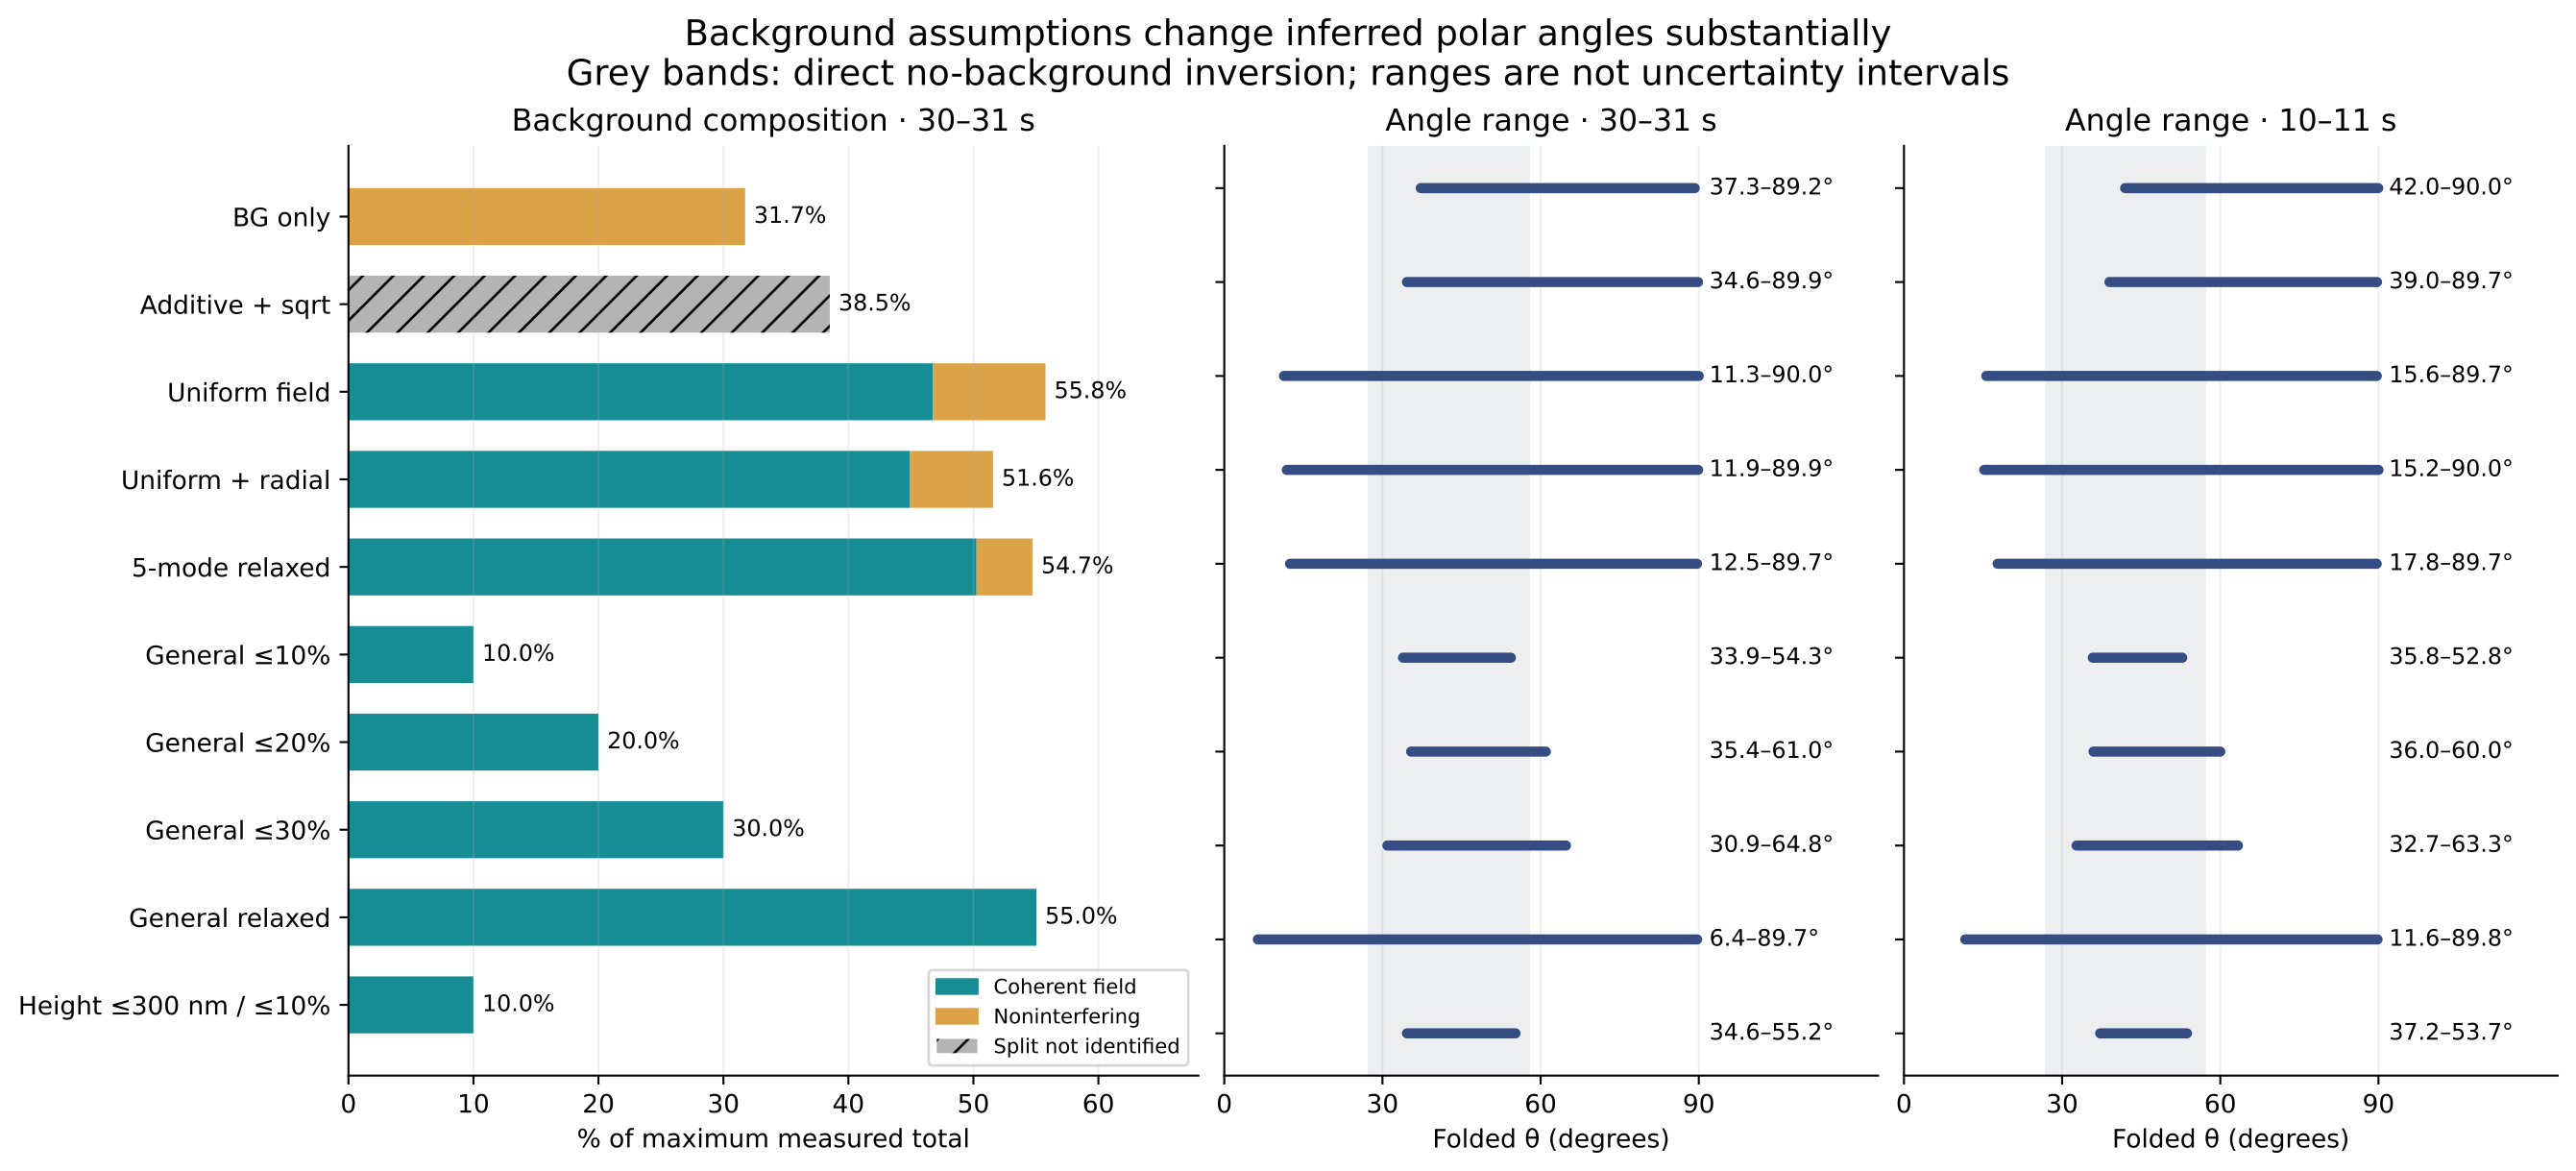
\includegraphics[width=\linewidth,height=3.35in,keepaspectratio]{figures/03_background_and_angles.png}\end{center}
Figure 3. Background is normalized to the maximum training total, T=\(\sum\)I\textsubscript{j}. The decomposition bars show 30–31 s; exact values for both windows are tabulated in the appendix. Grey angle bands show direct inversion. Changing the field family changes \(θ\) substantially, not just the residual.\par
The five-mode shared relaxed fit has B/Tmax=54.72\% / 54.43\% (30 s / 10 s). Its coherent share is 91.82\%, giving coherent power 50.25\% / 49.97\% of Tmax and noninterfering power 4.47\% / 4.45\%. In the general stationary and axial-motion selected fits, the residual Stokes component is effectively zero: essentially all fitted background is in the represented coherent field.\par
This split is conditional on the chosen mode space. “Noninterfering” can include light temporally incoherent with the rod, or coherent light spatially orthogonal to every signal mode being tested. Conversely, the represented coherent field can contain components with weak overlap at some orientations. Neither split assigns a percentage to coverslip, cell, objective or hole wall.\par
Historical “about 90–95\% background” referred to the \textbf{minimum} measured total in some earlier fits. It does not mean 90–95\% of the maximum. Both denominators are reported in the appendix. Nor does B\(\approx\)T at a dim point imply S\(\approx\)0 when C is negative: T=S+C+B, so destructive interference can conceal substantial rod-only power.\par
The unrestricted-overlap construction is deliberately excluded from these fitted-angle bars: it can reproduce the training curve exactly at a 10\% background budget, but it chooses overlap independently at each point. That demonstrates feasibility under weak bounds, not a valid stationary-field correction or validated angle recovery.\par
\clearpage
\heading{6. Power decomposition: why large background can survive}
\begin{center}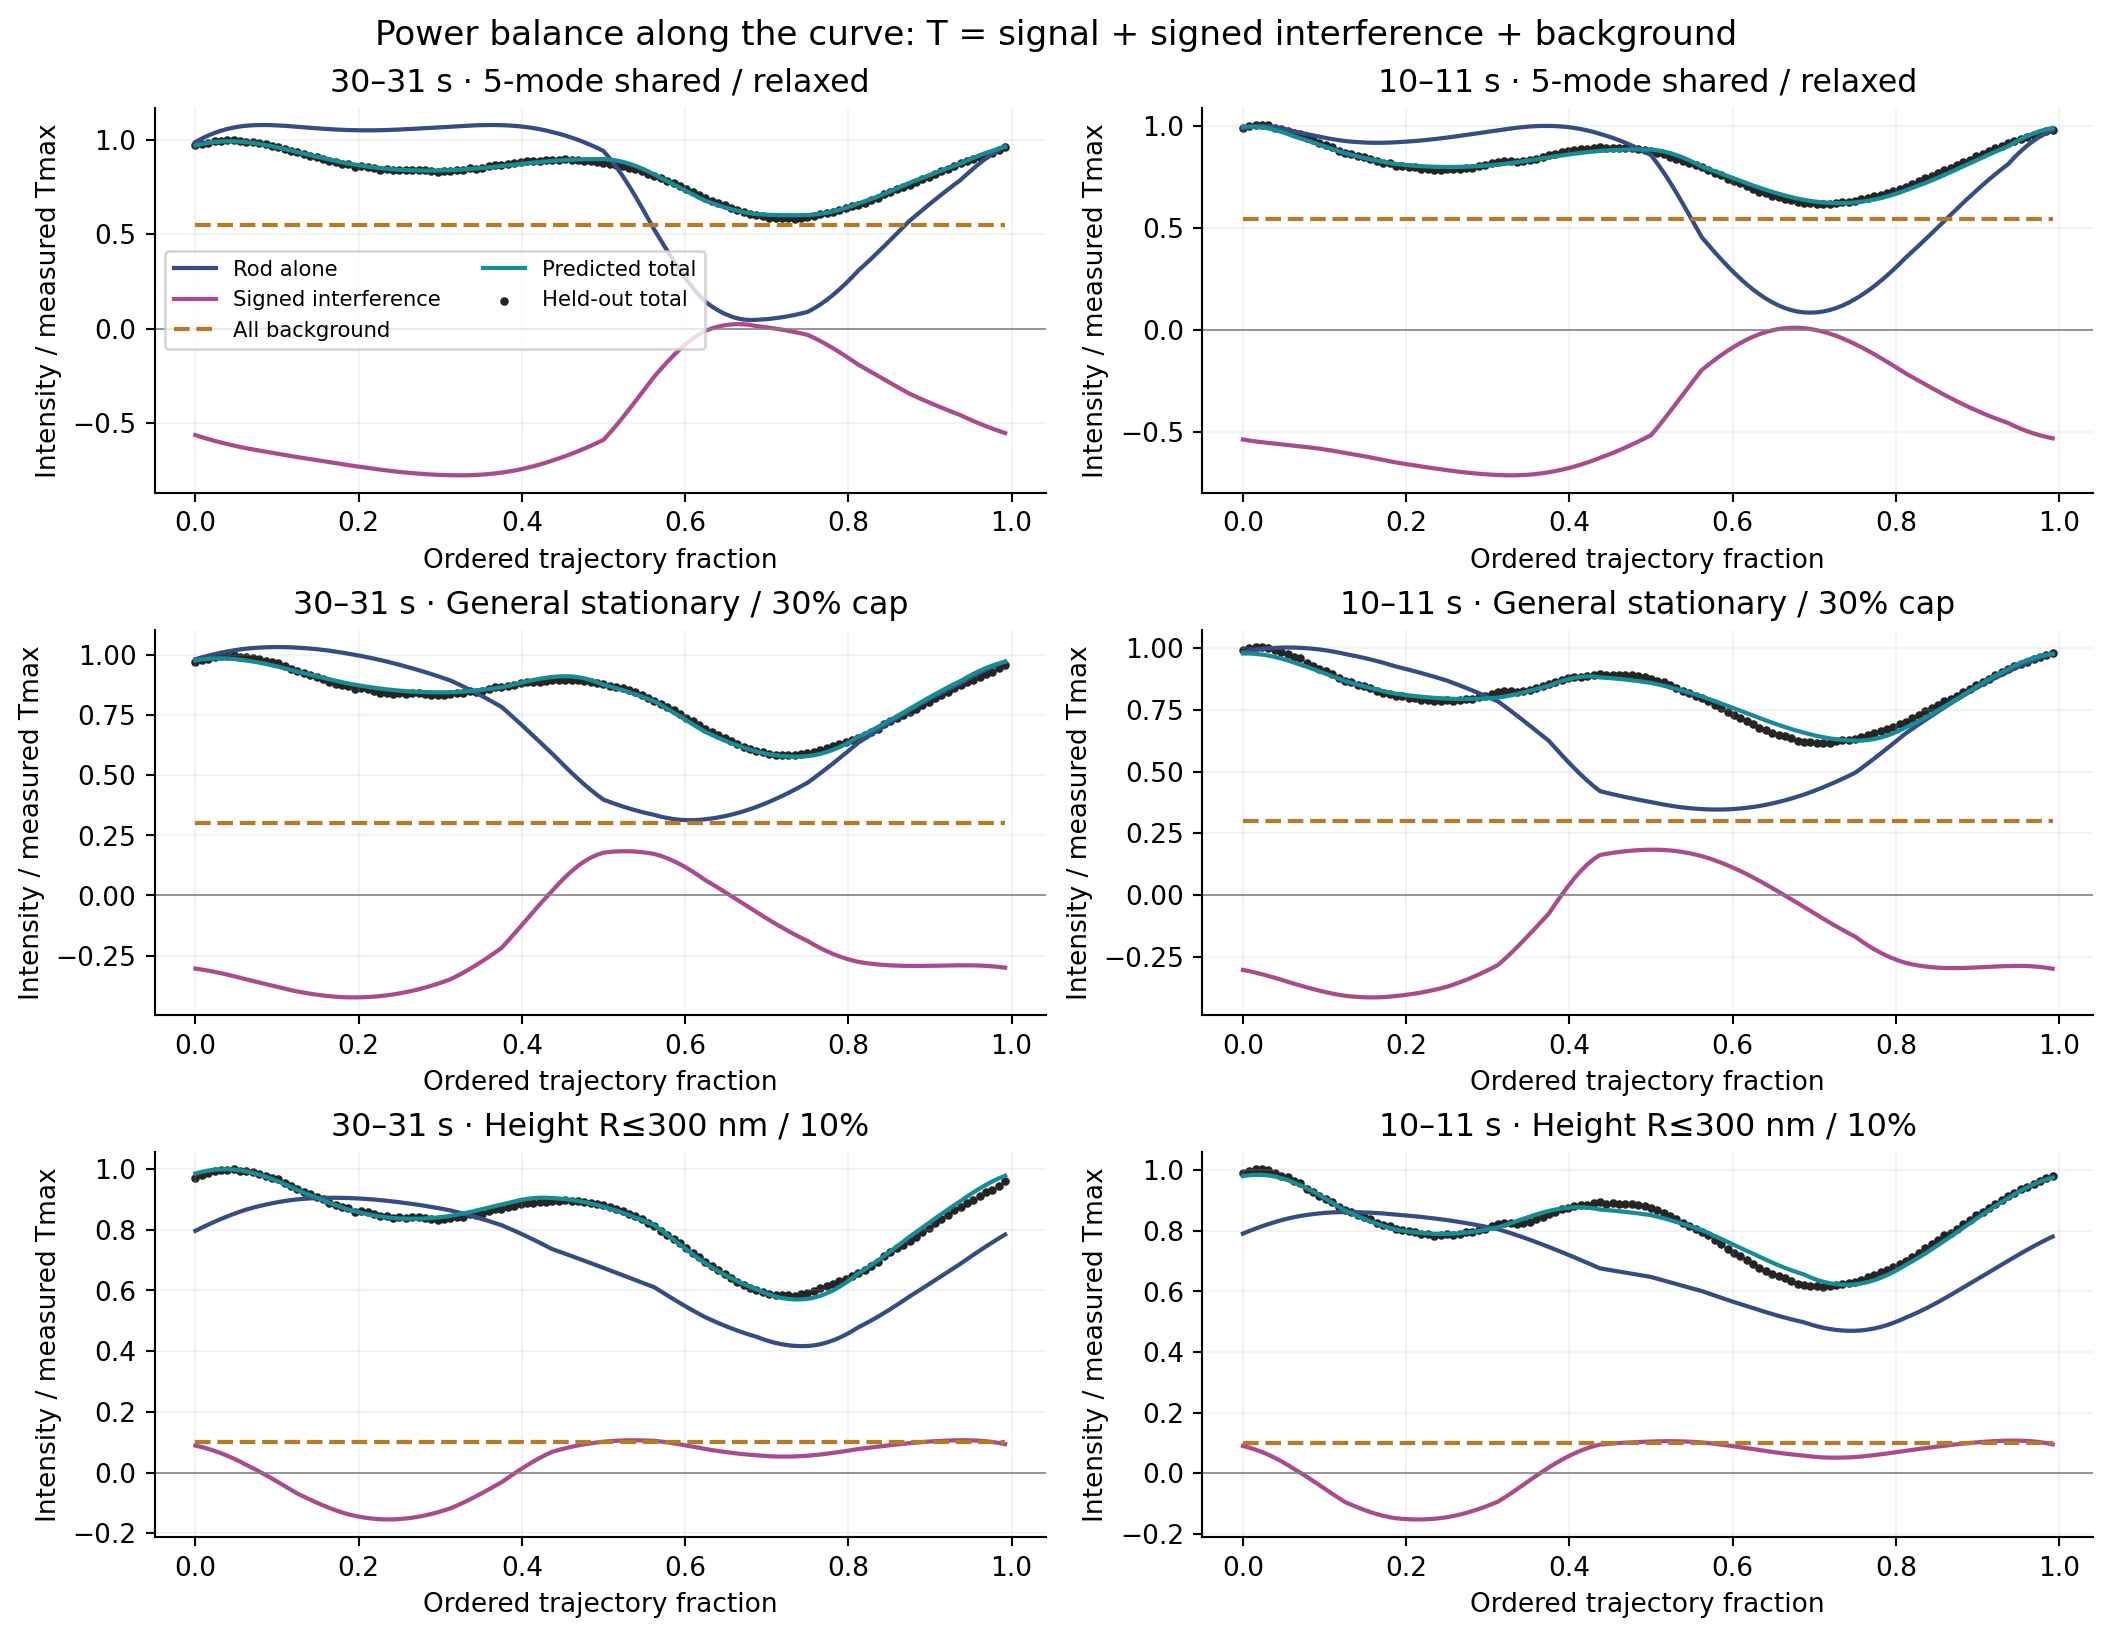
\includegraphics[width=\linewidth,height=5.5in,keepaspectratio]{figures/05_power_decomposition.png}\end{center}
Figure 5. All terms use the same Tmax normalization within each window. The rod-alone term obeys the one-a\textsubscript{0} excitation and collection law. The constant background and signed interference can compensate over substantial parts of the trajectory; the amount is not confined by an assumed positive “interference fraction.” Exact per-bin values are in comparison.json.\par
This checks the proposed intensity consistency condition: the recovered \(θ\) and the rod-only intensity use the same forward model and scale. Passing that internal consistency check does not establish the true \(θ\), because cone geometry, field overlap and background were jointly chosen. The general 30\% and moving-source 10\% examples redistribute the same observed power differently.\par
\clearpage
\heading{7. Angle variation along the trajectory}
\begin{center}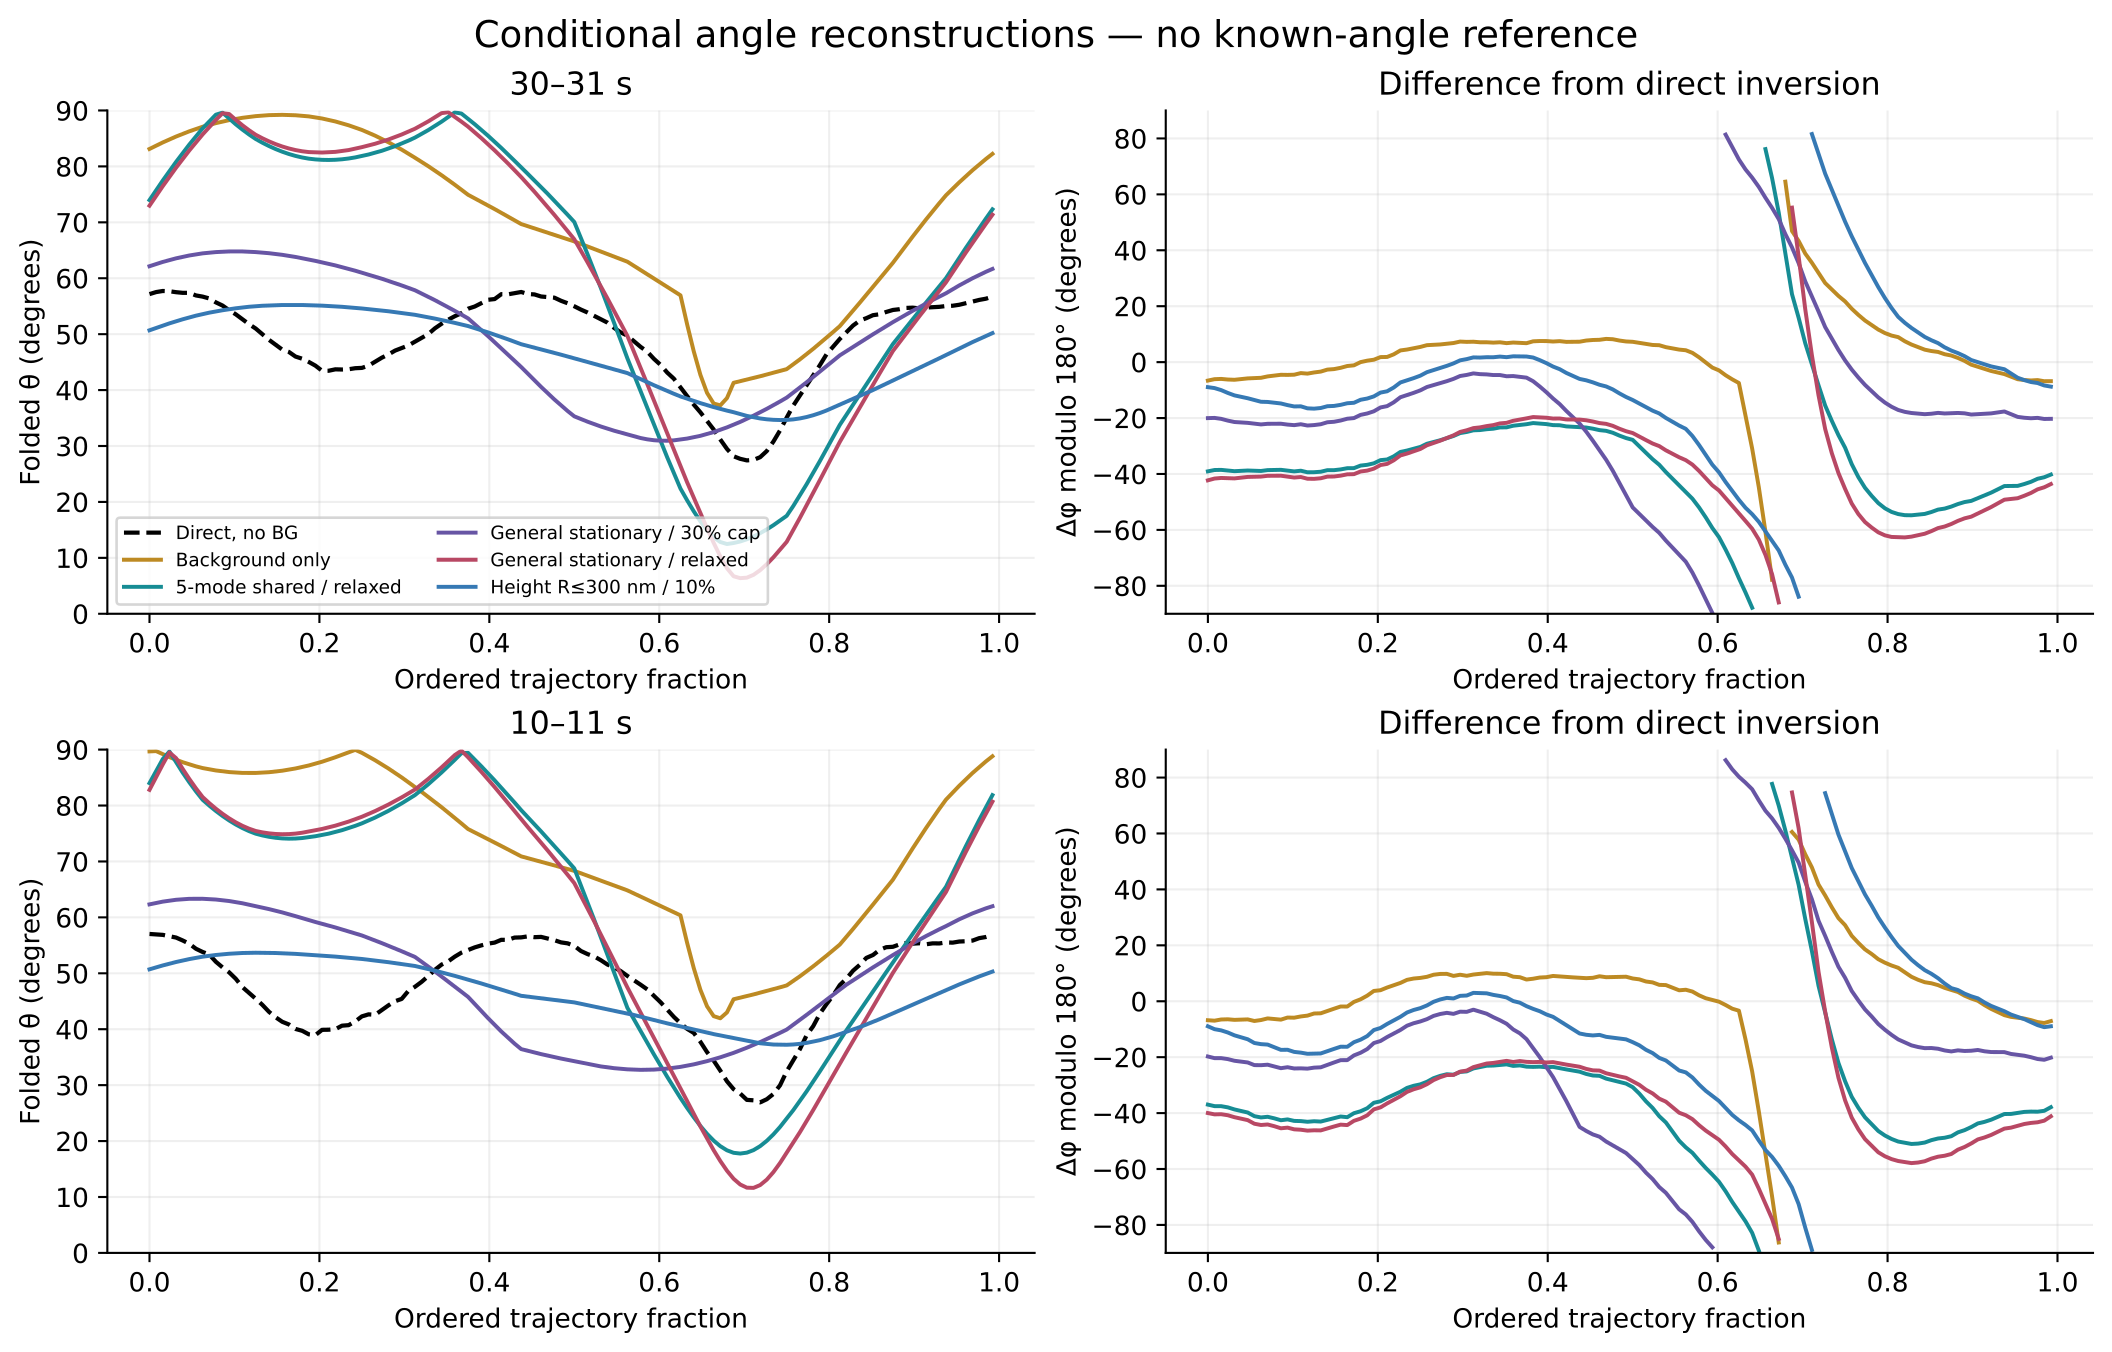
\includegraphics[width=\linewidth,height=4.75in,keepaspectratio]{figures/06_angle_traces.png}\end{center}
Figure 6. \(θ\) is folded to 0–90\textdegree{}. Azimuth differences are wrapped modulo 180\textdegree{}, with plot breaks at wrap discontinuities. These are comparisons at matched ordered bins, not errors relative to ground truth. Full \(θ\) and \(φ\) arrays, wrapped \(φ\) spans, and RMS differences from direct inversion are supplied in JSON/CSV.\par
The same measured curve admits fitted \(θ\) ranges extending almost to the equator in relaxed models, roughly 31–65\textdegree{} at the 30\% general stationary cap, or roughly 35–55\textdegree{} in the 300 nm axial-motion scenario. Near-90\textdegree{} solutions are especially sensitive to intensity/model errors. The evidence supports substantial angle ambiguity; it does not support choosing the narrowest or widest interval as more physical.\par
Do not interpret a wrapped \(φ\) minimum–maximum as a continuous rotation amplitude. The modulo-180\textdegree{} trace and branch-aware difference are the appropriate comparisons. A cone imposes continuity and a branch convention but does not add an independently known orientation.\par
\clearpage
\heading{8. Stationary-field completeness and the budget tradeoff}
\begin{center}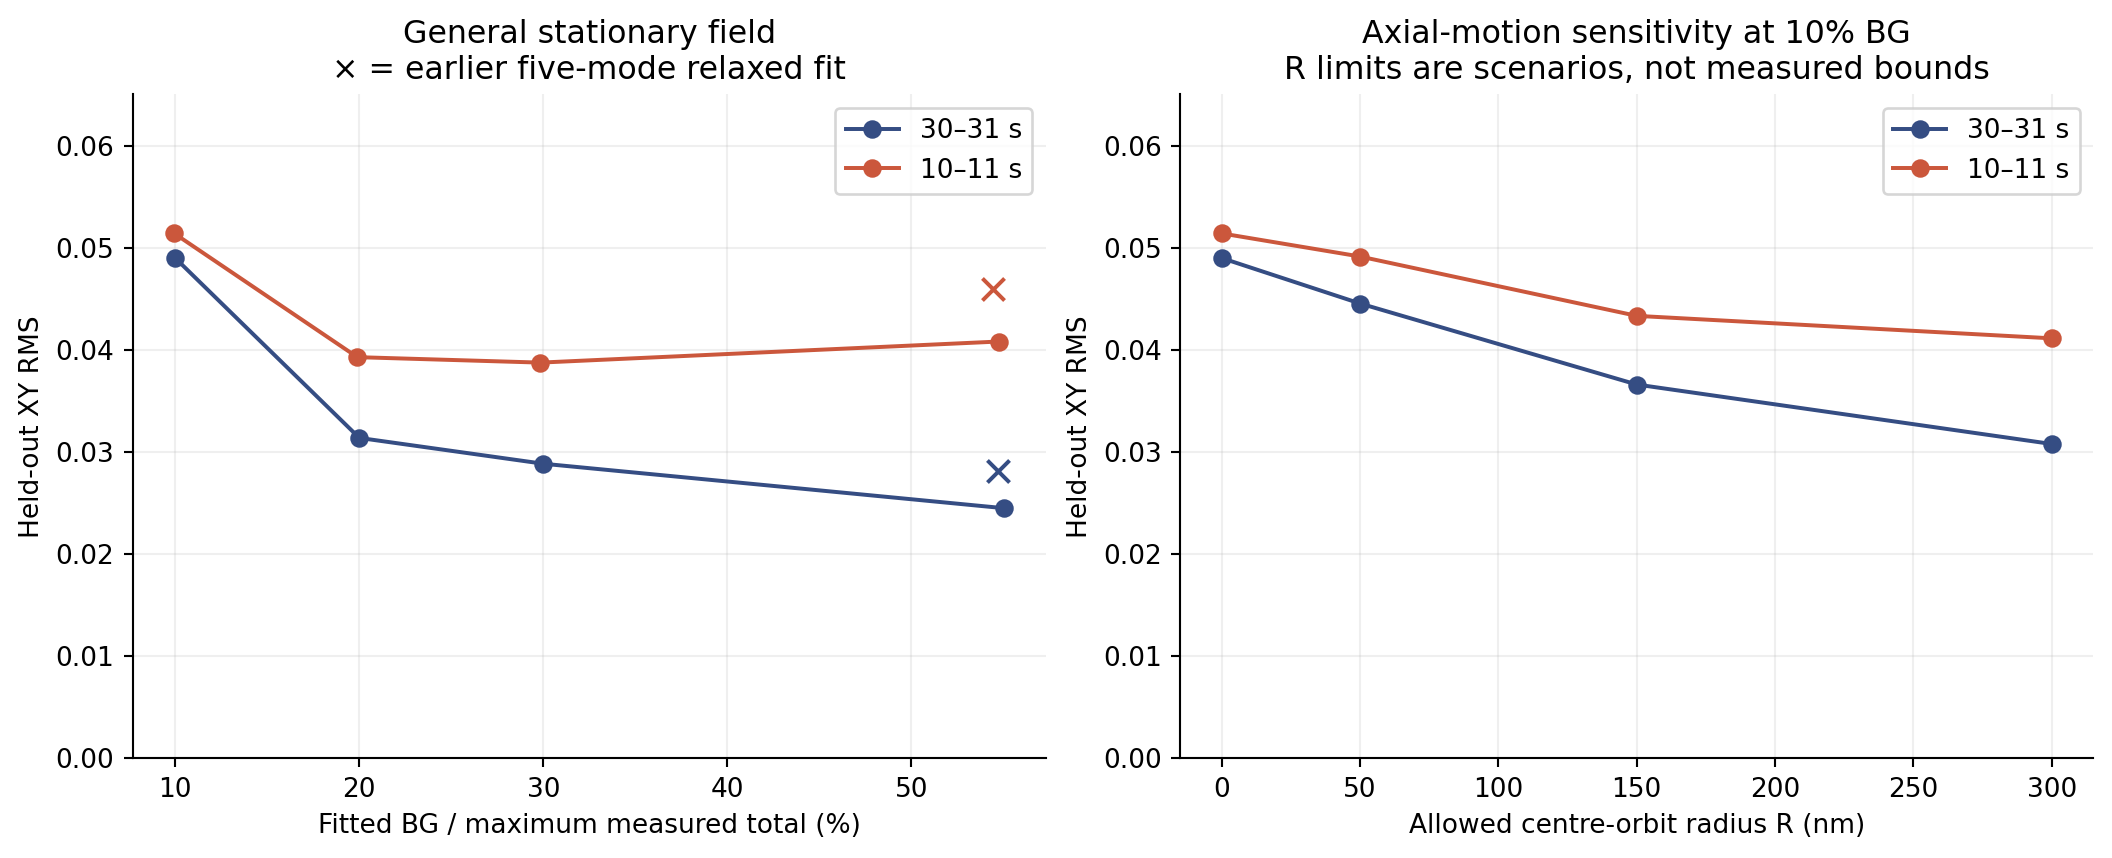
\includegraphics[width=\linewidth,height=2.8in,keepaspectratio]{figures/04_fit_tradeoffs.png}\end{center}
Figure 4. Left: selected general stationary fits versus their background budget, with the previous relaxed five-mode fit marked \(\times\). Right: adding bounded axial motion at 10\% background. The 10–11 s held-out residual need not decrease monotonically because optimization targets training channels, not held-out XY.\par
For a fixed-position ideal dipole, form the scalar span V of the x/y Cartesian components of its three collected dipole fields. Its numerical rank is five. Two transverse background components in V require ten complex coefficients. The Cartesian remainder is orthogonal to V: it has no interference with any signal orientation and no integrated cross term with the represented field. Its observable residual intensity is captured by three positive Stokes parameters.\par
This supplies a complete observation representation for a \textbf{stationary common-pupil field under the fixed-position, ideal-dipole, full-collection assumptions}. Ten is a sufficient mode count, not a count of physical scattering objects or uniquely identifiable coefficients. Basis-dependent modal powers should not be labeled as specific sources. Adding further stationary pupil modes cannot improve this ideal fixed-position model beyond that representation.\par
With the circular-excitation law, the stationary rod–background cross term is quadratic in the direction d: on a fixed cone it contains mechanical-phase harmonics only through order two. Rod-only intensity is quartic and can contain order four. This restriction is why an arbitrary overlap at every bin is much more permissive than a stationary field.\par
The fit remains nonconvex in cone, phase and field parameters. Reported minima are feasible examples from the saved multistart searches, not proofs that a lower budget is impossible. Independent post-analyzer backgrounds, calibration errors, non-dipolar response, changing excitation and moving-source effects fall outside the completeness claim. Alternate-cycle agreement alone does not resolve them.\par
\clearpage
\heading{9. Hole shape, localized scattering and bounded height}
\begin{center}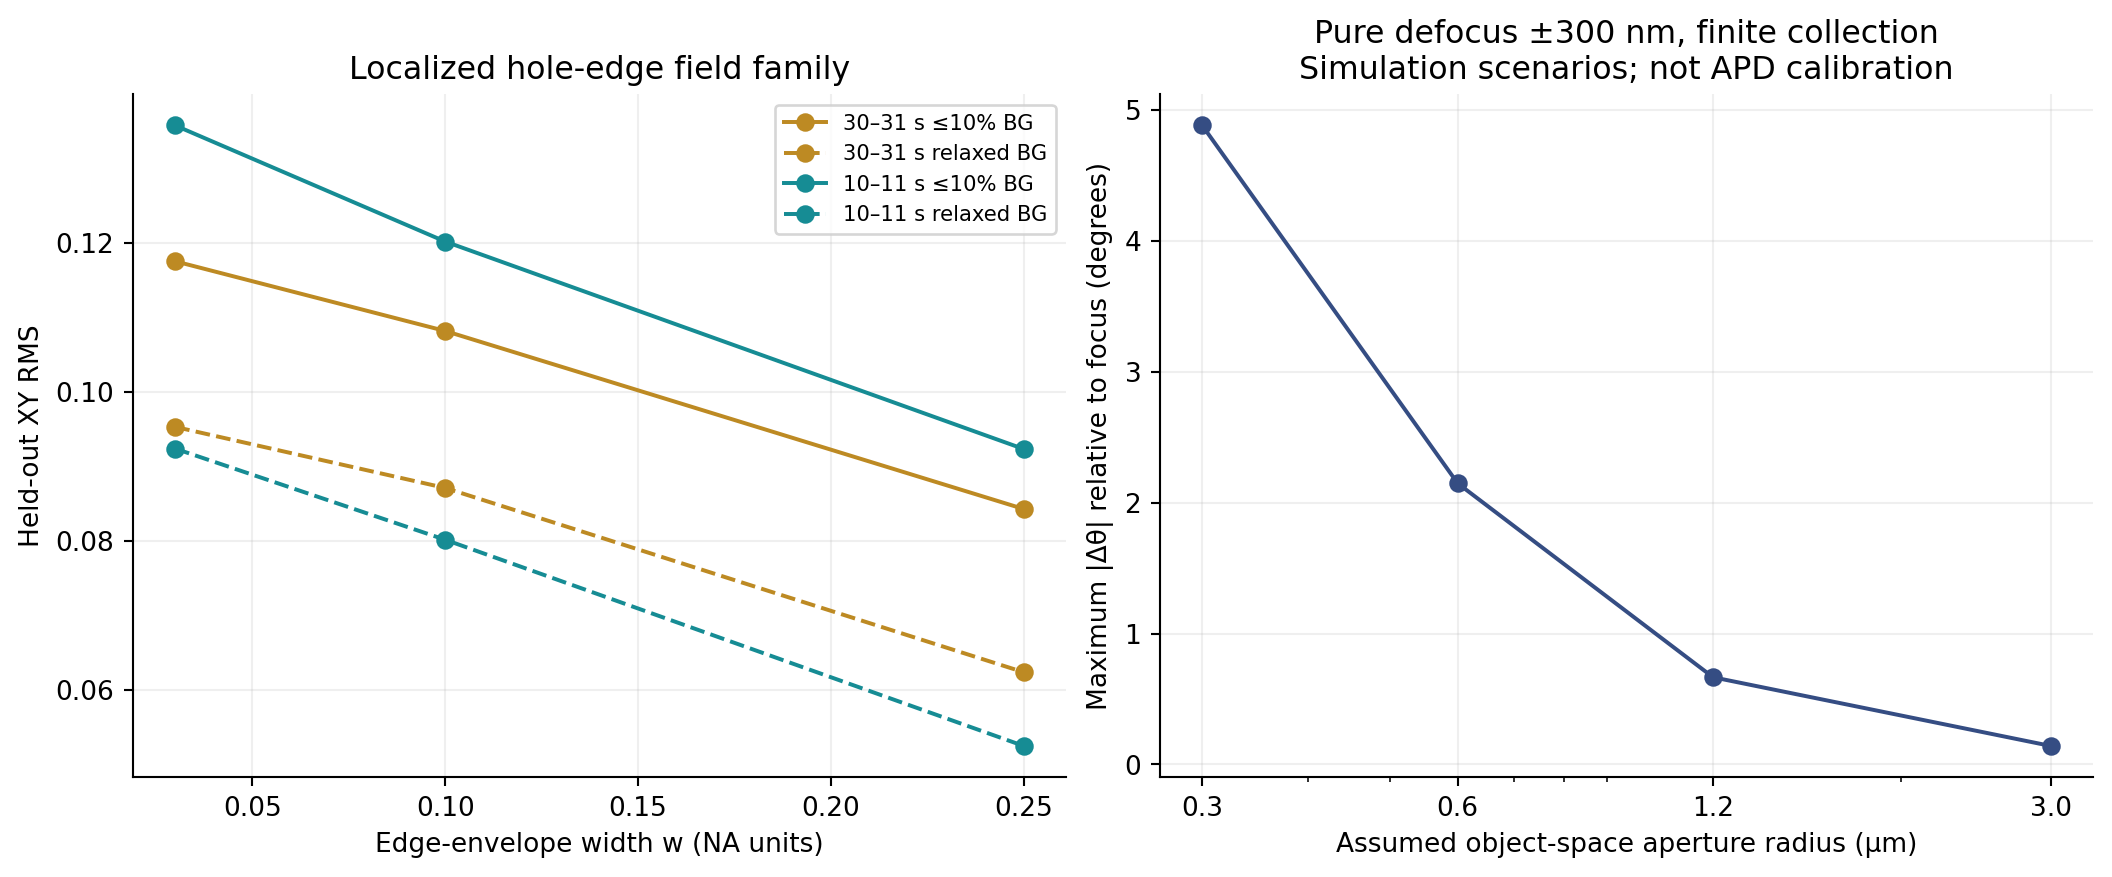
\includegraphics[width=\linewidth,height=2.8in,keepaspectratio]{figures/07_edge_and_focus.png}\end{center}
Figure 7. Left: six complex edge-field coefficients, shared across windows, with Gaussian radial envelope exp[\(-\)(\(ρ\)\(-\)0.38)\textsuperscript{2}/(2w\textsuperscript{2})] multiplied by 1, cos\(ϕ\), sin\(ϕ\) in each transverse polarization. Widths 0.03, 0.10 and 0.25 NA were tested. Narrow fields fit poorly; broader fields improve but become less specifically localized to the edge. The narrow 10\% selected run reached its evaluation limit; it is not a converged exclusion result.\par
This is an effective low-order field family, not a Maxwell calculation of the drilled wall. Wall topography, coating, mirror tilt and distance from the true BFP are not known. It cannot rule out all hole scattering. Separately, using the thesis measured amplitude mask at four rotations changed held-out XY RMS by less than about 0.0002 in the three-mode comparisons. That tests pupil transmission shape, not edge scattering or out-of-BFP propagation.\par
Axial-motion model: z(\(χ\))=R sin(\(θ\)\textsubscript{axis})cos(\(χ\)+\(δ\)), with R and \(δ\) independent per window. R is not the rod-orientation cone radius or assumed rod length. Caps 50, 150 and 300 nm are sensitivity scenarios, not biological measurements. The 300 nm fits use R\(\approx\)228 / 300 nm, but axial amplitudes only 40.7 / 43.0 nm (about 81 / 86 nm peak-to-peak). Boundary-hitting radii warn against treating them as recovered hook geometry.\par
The rod field acquires axial phase exp[i(2\(π\)/\(λ\))z(n\textsubscript{w}+\(\surd\)(n\textsubscript{w}\textsuperscript{2}\(-\)\(ρ\)\textsuperscript{2}))], \(λ\)=633 nm, including incident and collected propagation. A Gaussian illumination with 2 \(\mu\)m Rayleigh range and its Gouy phase is assumed. At the selected amplitudes its intensity change is below 0.05\%; phase-dependent interference, rather than brightness loss, drives most of this fitted improvement.\par
Only axial motion is modeled; lateral motion, uncertain mean height, interface-dependent rod response and finite APD acceptance are not fitted jointly. Once the source moves, the ten-mode background is a restricted family again; fixed-position completeness no longer applies. The separate pure-defocus aperture simulation on the right tests \(\pm\)300 nm and several orientations, without background. Full collection conserves power; clipping can alter \(θ\). These aperture radii are not calibrated APD sizes.\par
\clearpage
\heading{10. Physical interpretation and the useful stopping line}
\textbf{Background categories from Richard’s correspondence.} External optical reflections/scattering can carry arbitrary phase and spatial structure. Ideal coverslip reflection should leave through the central hole. Any reflected light that remains after bouncing or scattering need not retain a simple circular-polarization phase relation. Cell scattering can come from different heights and different polarization components; nearby rods add sample-associated fields. The APD integrates their overlap, so equal source position for the rod does not imply equal interference phase in all channels.\par
Multiple mutually coherent stationary backgrounds add as fields before squaring. If they lie in the same allowed mode space, fitting two copies does not add a new observation model; it only makes the decomposition redundant. Mutually incoherent contributions add intensities. More sources become observationally distinct when they add new spatial/polarization modes, different coherence, motion or a response to an experimental perturbation. Their source locations cannot generally be inferred from one steady four-channel trajectory.\par
Fresnel transmission, BFP mapping and the hole act on fields along the optical path; a source should enter where it is generated. After propagation to one common detection plane, the background can be represented there for this effective model. Intensity subtraction is not generally a commuting substitute for coherent propagation. The present fits do not identify which optical surface produced the effective field.\par
\textbf{What the existing data can do:} reject or expose poor versions of restricted model families; show budget–angle sensitivity; check shared-field consistency across windows; quantify registration and chronological variation; test whether physically linked terms reproduce channels as well as the outline. It cannot establish unique absolute \(θ\), actual coherent source fractions, APD acceptance, or true centre motion without additional constraints.\par
\textbf{Priority discussion with Richard:} which perturbation best separates stationary optical field from sample-associated field in this APD setup? An axial stage scan/modulation with four-channel acquisition is especially direct, provided rod orientation, position and exposure averaging are tracked. It can constrain a phase-dependent cross term; it is not automatically an exact background subtraction.\par
Fixed-rod files can quantify temporal stability, channel covariance, spectra and response to laser-power steps. Flat intensity alone cannot bound a static coherent background. A nearly constant-\(θ\) rotating rod can test azimuth-dependent power and shared-field predictions, but its circular anisotropy provides less leverage for separating additive scale/background. These are useful controls, not substitutes for known-angle truth.\par
Other discriminating measurements are dark electronic offsets, a current transmission/mixing calibration, effective APD acceptance/defocus scans, and centre-position tracking. The sensible next step is to pick one or two constraints, not add another unconstrained per-bin term. A synthetic injection/recovery study can characterize an estimator under assumed models, but would not decide which model describes this old sample.\par
\clearpage
\heading{11. Source limits, verification and reproducible record}
\textbf{Bearing paper and SI.} The supplied manuscript and supplementary-information (1).pdf describe deliberately selected near-axis rods with overlapping loops, fewer than 10\% of candidates. Do not transfer that geometry or biological conclusions to ordinary BFM samples. SI S1 documents the drilled mirror near an inaccessible BFP, hole-wall scattering, polarization/alignment issues and APD alignment. SI p5 transmission/extinction values are historical, not a current calibration. Fixed-rod noise measurements and manual azimuth tests establish precision/\(φ\) behavior, not exact \(θ\) or a coherent-background bound.\par
\textbf{Polarcam draft and SI.} Polarcam Manuscript V2 2026-09-08 RB.docx, SI outline.docx and RB Figs V2.docx were reviewed separately. Their camera background values, compensation optics, exposure/modulation behavior and some placeholder numbers are not transferred to this APD data. Axial modulation and lateral minimum projection motivate discriminating tests but require their own assumptions. APD on the Polarcam setup is not the bearing-paper APD setup.\par
\textbf{Thesis and optical sources.} Thesis sections 1.5–1.8 and its measured mirror mask supplied optical context; mask provenance is thesis commit 7576b50, analysis/image\_mirror\_binary.tif. The active baseline remains NA\textsubscript{in}=0.38. Original notebook fitting history was recovered from repository import 9b3604e. The model conventions and dated source notes accompany the scripts. General pupil-phase context: \url{https://pmc.ncbi.nlm.nih.gov/articles/PMC5810908/} ; the present calculation uses water-side propagation with the existing water–oil transmission.\par
\textbf{Numerical checks.} This report reconstructs and checks 46 model/window predictions against saved residuals and checks S+C+B consistency. Earlier checks reproduce all 15 saved edge/general/height comparisons; arbitrary fixed-field overlap projection error is about 2.9\(\times\)10\textsuperscript{-16}; pupil refinement changes channels by about 1.2\(\times\)10\textsuperscript{-4} for general fields and 7.2\(\times\)10\textsuperscript{-4} for the narrow edge family; checked axial interpolation error is about 5.3\(\times\)10\textsuperscript{-7}. These are numerical checks, not experimental accuracy bounds.\par
The best narrow-edge 10\% run has success=false at 600 function evaluations. Other selected runs in the principal table meet their optimizer termination criteria. Several caps/radius constraints are active, and multistart optimization does not certify global minima. No information criterion or formal confidence interval is claimed: correlated bins, estimated registration and unknown error covariance make naive parameter-count significance unreliable.\par
\textbf{Reproduction.} comparison.csv is a compact numerical table; comparison.json includes per-bin predictions, signal/interference/background decomposition, training/test arrays and angles. build\_data.py reconstructs results; plot\_figures.py draws seven PNG/SVG figure sets; build\_report.py creates this PDF and editable Word document. The study archive preserves earlier scripts, fit parameters, cached averages, optical inputs and dated notes. Replotting cached results does not require the large raw TDMS. Reprocessing and refitting require their documented data paths and dependencies.\par
No future Codex handoff script is included yet. The code and dated record are the current milestone; the report is intended to settle the scientific next step before extending the model.\par
\clearpage
\heading{Appendix A · 30–31 s: fit quality and angles}
{\footnotesize\setlength{\tabcolsep}{4pt}\begin{tabularx}{\linewidth}{>{\hsize=2.468\hsize}Y>{\hsize=0.693\hsize}Y>{\hsize=0.722\hsize}Y>{\hsize=0.693\hsize}Y>{\hsize=0.967\hsize}Y>{\hsize=0.852\hsize}Y>{\hsize=0.606\hsize}Y}\toprule\rowcolor{pale}
\textbf{Model} & \textbf{XY RMS} & \textbf{Channel\newline RMS \%} & \textbf{Total\newline RMS \%} & \textbf{\(θ\) span (\textdegree{})} & \textbf{\(φ\) RMS vs\newline direct (\textdegree{})} & \textbf{Param.}\\\midrule
Background only & 0.0896 & 2.29 & 5.81 & 37.3–89.2 & 17.5 & 23 L\\
Additive + sqrt extension & 0.0927 & 2.14 & 4.80 & 34.6–89.9 & 18.2 & 27 L\\
Uniform field (2 modes) & 0.0538 & 1.05 & 2.25 & 11.3–90.0 & 41.4 & 27 L\\
Uniform + radial (3 modes) & 0.0317 & 0.60 & 0.98 & 11.9–89.9 & 39.7 & 29 L\\
3-mode shared / relaxed & 0.0336 & 0.65 & 1.26 & 11.1–89.8 & 40.3 & 49 S\\
3-mode shared / 10\% cap & 0.0950 & 2.15 & 4.88 & 26.6–53.9 & 19.3 & 49 S\\
5-mode shared / relaxed & 0.0281 & 0.59 & 1.15 & 12.5–89.7 & 41.5 & 53 S\\
5-mode shared / 10\% cap & 0.0930 & 2.11 & 4.75 & 26.4–53.8 & 19.5 & 53 S\\
Edge w=0.03 / 10\% cap & 0.1175 & 2.66 & 5.97 & 36.2–57.3 & 16.8 & 52 S *\\
Edge w=0.03 / relaxed & 0.0953 & 2.03 & 4.63 & 33.7–88.6 & 19.5 & 52 S\\
Edge w=0.1 / 10\% cap & 0.1082 & 2.45 & 5.53 & 34.5–56.5 & 18.7 & 52 S\\
Edge w=0.1 / relaxed & 0.0871 & 1.87 & 4.39 & 35.8–79.6 & 21.3 & 52 S\\
Edge w=0.25 / 10\% cap & 0.0843 & 1.93 & 4.50 & 33.1–55.4 & 20.0 & 52 S\\
Edge w=0.25 / relaxed & 0.0624 & 1.36 & 3.23 & 36.7–66.7 & 25.8 & 52 S\\
General stationary / 10\% cap & 0.0490 & 1.06 & 2.74 & 33.9–54.3 & 26.0 & 63 S\\
General stationary / relaxed & 0.0245 & 0.49 & 0.87 & 6.4–89.7 & 42.6 & 63 S\\
General stationary / 20\% cap & 0.0314 & 0.67 & 1.52 & 35.4–61.0 & 31.6 & 63 S\\
General stationary / 30\% cap & 0.0288 & 0.62 & 1.36 & 30.9–64.8 & 34.2 & 63 S\\
Height R\(\leq\)50 nm / 10\% & 0.0445 & 0.94 & 2.40 & 34.3–54.8 & 26.1 & 67 S\\
Height R\(\leq\)150 nm / 10\% & 0.0366 & 0.75 & 1.80 & 33.8–56.2 & 27.0 & 67 S\\
Height R\(\leq\)300 nm / 10\% & 0.0308 & 0.64 & 1.39 & 34.6–55.2 & 28.5 & 67 S\\
\bottomrule\end{tabularx}}\par\medskip
Channel and total RMS use residual divided by observed total at each bin; channel RMS is not relative to each channel individually. \(θ\) span covers the sampled fitted orientations. \(φ\) differences use modulo 180\textdegree{}. S = total parameters in the joint two-window fit; L = parameters in this separate single-window fit. * = selected run reached its evaluation limit. Numeric termination does not establish global optimality.\par
Direct no-background inversion is not a fitted cone and has no fitted prediction score here. All historical and verified duplicates are retained in comparison.json/CSV. Early free-brightness and arbitrary-overlap constructions are not comparable predictive models and are intentionally kept outside this table.\par
\clearpage
\heading{Appendix B · 30–31 s: background composition}
{\footnotesize\setlength{\tabcolsep}{4pt}\begin{tabularx}{\linewidth}{>{\hsize=2.128\hsize}Y>{\hsize=0.619\hsize}Y>{\hsize=0.619\hsize}Y>{\hsize=0.705\hsize}Y>{\hsize=0.680\hsize}Y>{\hsize=1.249\hsize}Y}\toprule\rowcolor{pale}
\textbf{Model} & \textbf{All BG\newline \% Tmax} & \textbf{All BG\newline \% Tmin} & \textbf{Coherent\newline \% Tmax} & \textbf{Residual\newline \% Tmax} & \textbf{Channel BG \% Tmax\newline 0 / 90 / 45 / 135}\\\midrule
Background only & 31.74 & 54.07 & 0.0 & 31.7 & 9.3/6.6/4.7/11.1\\
Additive + sqrt extension & 38.51 & 65.60 & — & — & 13.5/5.7/9.1/10.2\\
Uniform field (2 modes) & 55.77 & 95.00 & 46.8 & 9.0 & 15.4/12.5/10.4/17.5\\
Uniform + radial (3 modes) & 51.57 & 87.85 & 44.9 & 6.6 & 16.1/9.7/9.7/16.0\\
3-mode shared / relaxed & 53.05 & 90.37 & 46.2 & 6.9 & 16.8/9.7/9.9/16.7\\
3-mode shared / 10\% cap & 10.00 & 17.04 & 4.3 & 5.7 & 4.2/0.8/1.3/3.7\\
5-mode shared / relaxed & 54.72 & 93.23 & 50.3 & 4.5 & 17.9/9.4/10.6/16.7\\
5-mode shared / 10\% cap & 10.00 & 17.04 & 5.5 & 4.5 & 4.1/0.9/1.5/3.5\\
Edge w=0.03 / 10\% cap & 10.00 & 17.04 & 10.0 & 0.0 & 3.5/1.5/0.4/4.6\\
Edge w=0.03 / relaxed & 34.90 & 59.46 & 34.9 & 0.0 & 11.5/5.9/6.7/10.8\\
Edge w=0.1 / 10\% cap & 10.00 & 17.04 & 10.0 & 0.0 & 4.1/0.9/1.0/4.0\\
Edge w=0.1 / relaxed & 31.90 & 54.35 & 31.9 & 0.0 & 10.9/5.1/5.8/10.2\\
Edge w=0.25 / 10\% cap & 10.00 & 17.04 & 10.0 & 0.0 & 4.3/0.7/1.3/3.7\\
Edge w=0.25 / relaxed & 25.63 & 43.66 & 25.6 & 0.0 & 9.8/3.1/4.0/8.8\\
General stationary / 10\% cap & 10.00 & 17.04 & 10.0 & 0.0 & 4.1/0.9/1.3/3.7\\
General stationary / relaxed & 55.04 & 93.76 & 55.0 & 0.0 & 17.3/10.3/11.3/16.3\\
General stationary / 20\% cap & 20.00 & 34.07 & 20.0 & 0.0 & 9.0/1.0/3.0/7.0\\
General stationary / 30\% cap & 30.00 & 51.11 & 30.0 & 0.0 & 12.2/2.8/4.3/10.7\\
Height R\(\leq\)50 nm / 10\% & 10.00 & 17.04 & 10.0 & 0.0 & 4.1/0.9/1.3/3.7\\
Height R\(\leq\)150 nm / 10\% & 10.00 & 17.04 & 10.0 & 0.0 & 4.0/1.0/1.0/4.0\\
Height R\(\leq\)300 nm / 10\% & 10.00 & 17.04 & 10.0 & 0.0 & 3.8/1.2/0.9/4.1\\
\bottomrule\end{tabularx}}\par\medskip
Tmax and Tmin are from the training total within this window. Channel entries sum to all BG up to rounding. Coherent/residual components are nonnegative fitted powers; interference is signed and reported separately in Figure 5 and comparison.json. A dash means the effective model does not identify that split. Near-zero residual components are rounded to 0.0\%; this is a model-dependent boundary solution, not proof that all real background is coherent.\par
Shared-field coefficients are identical in absolute units between windows. Their percentages differ because the observed maxima/minima differ. The background is constant along each fitted trajectory; it is the signal–background cross term that varies with orientation and, in the height scenario, position.\par
\clearpage
\heading{Appendix A · 10–11 s: fit quality and angles}
{\footnotesize\setlength{\tabcolsep}{4pt}\begin{tabularx}{\linewidth}{>{\hsize=2.468\hsize}Y>{\hsize=0.693\hsize}Y>{\hsize=0.722\hsize}Y>{\hsize=0.693\hsize}Y>{\hsize=0.967\hsize}Y>{\hsize=0.852\hsize}Y>{\hsize=0.606\hsize}Y}\toprule\rowcolor{pale}
\textbf{Model} & \textbf{XY RMS} & \textbf{Channel\newline RMS \%} & \textbf{Total\newline RMS \%} & \textbf{\(θ\) span (\textdegree{})} & \textbf{\(φ\) RMS vs\newline direct (\textdegree{})} & \textbf{Param.}\\\midrule
Background only & 0.0989 & 2.56 & 6.66 & 42.0–90.0 & 19.5 & 23 L\\
Additive + sqrt extension & 0.1024 & 2.41 & 4.95 & 39.0–89.7 & 18.2 & 27 L\\
Uniform field (2 modes) & 0.0709 & 1.30 & 1.69 & 15.6–89.7 & 41.8 & 27 L\\
Uniform + radial (3 modes) & 0.0495 & 1.01 & 1.76 & 15.2–90.0 & 42.7 & 29 L\\
3-mode shared / relaxed & 0.0509 & 1.04 & 1.69 & 16.1–89.9 & 41.7 & 49 S\\
3-mode shared / 10\% cap & 0.1040 & 2.36 & 4.86 & 29.2–52.1 & 18.9 & 49 S\\
5-mode shared / relaxed & 0.0460 & 0.98 & 1.68 & 17.8–89.7 & 42.4 & 53 S\\
5-mode shared / 10\% cap & 0.1019 & 2.32 & 4.78 & 29.0–52.0 & 19.1 & 53 S\\
Edge w=0.03 / 10\% cap & 0.1357 & 3.14 & 6.60 & 37.9–54.2 & 17.7 & 52 S *\\
Edge w=0.03 / relaxed & 0.0924 & 2.17 & 4.76 & 39.5–90.0 & 18.7 & 52 S\\
Edge w=0.1 / 10\% cap & 0.1202 & 2.79 & 5.76 & 36.9–53.7 & 17.9 & 52 S\\
Edge w=0.1 / relaxed & 0.0802 & 1.97 & 4.62 & 41.8–78.6 & 20.9 & 52 S\\
Edge w=0.25 / 10\% cap & 0.0923 & 2.19 & 4.72 & 35.5–52.9 & 19.3 & 52 S\\
Edge w=0.25 / relaxed & 0.0525 & 1.48 & 3.96 & 40.4–64.1 & 25.7 & 52 S\\
General stationary / 10\% cap & 0.0514 & 1.33 & 3.62 & 35.8–52.8 & 26.0 & 63 S\\
General stationary / relaxed & 0.0408 & 0.91 & 1.92 & 11.6–89.8 & 43.1 & 63 S\\
General stationary / 20\% cap & 0.0393 & 1.03 & 2.65 & 36.0–60.0 & 34.7 & 63 S\\
General stationary / 30\% cap & 0.0387 & 0.99 & 2.47 & 32.7–63.3 & 38.3 & 63 S\\
Height R\(\leq\)50 nm / 10\% & 0.0491 & 1.24 & 3.24 & 36.4–53.4 & 26.1 & 67 S\\
Height R\(\leq\)150 nm / 10\% & 0.0433 & 1.10 & 2.76 & 36.4–54.6 & 27.1 & 67 S\\
Height R\(\leq\)300 nm / 10\% & 0.0411 & 0.99 & 2.19 & 37.2–53.7 & 27.9 & 67 S\\
\bottomrule\end{tabularx}}\par\medskip
Channel and total RMS use residual divided by observed total at each bin; channel RMS is not relative to each channel individually. \(θ\) span covers the sampled fitted orientations. \(φ\) differences use modulo 180\textdegree{}. S = total parameters in the joint two-window fit; L = parameters in this separate single-window fit. * = selected run reached its evaluation limit. Numeric termination does not establish global optimality.\par
Direct no-background inversion is not a fitted cone and has no fitted prediction score here. All historical and verified duplicates are retained in comparison.json/CSV. Early free-brightness and arbitrary-overlap constructions are not comparable predictive models and are intentionally kept outside this table.\par
\clearpage
\heading{Appendix B · 10–11 s: background composition}
{\footnotesize\setlength{\tabcolsep}{4pt}\begin{tabularx}{\linewidth}{>{\hsize=2.128\hsize}Y>{\hsize=0.619\hsize}Y>{\hsize=0.619\hsize}Y>{\hsize=0.705\hsize}Y>{\hsize=0.680\hsize}Y>{\hsize=1.249\hsize}Y}\toprule\rowcolor{pale}
\textbf{Model} & \textbf{All BG\newline \% Tmax} & \textbf{All BG\newline \% Tmin} & \textbf{Coherent\newline \% Tmax} & \textbf{Residual\newline \% Tmax} & \textbf{Channel BG \% Tmax\newline 0 / 90 / 45 / 135}\\\midrule
Background only & 34.62 & 55.81 & 0.0 & 34.6 & 9.8/7.5/4.7/12.6\\
Additive + sqrt extension & 39.93 & 64.38 & — & — & 14.0/6.0/9.8/10.2\\
Uniform field (2 modes) & 58.92 & 95.00 & 45.6 & 13.3 & 17.1/12.3/10.5/19.0\\
Uniform + radial (3 modes) & 55.34 & 89.23 & 47.9 & 7.4 & 17.6/10.1/10.1/17.6\\
3-mode shared / relaxed & 52.76 & 85.07 & 45.9 & 6.8 & 16.7/9.7/9.8/16.6\\
3-mode shared / 10\% cap & 9.95 & 16.04 & 4.3 & 5.7 & 4.2/0.8/1.3/3.6\\
5-mode shared / relaxed & 54.43 & 87.75 & 50.0 & 4.4 & 17.8/9.4/10.6/16.7\\
5-mode shared / 10\% cap & 9.95 & 16.04 & 5.5 & 4.5 & 4.1/0.9/1.5/3.5\\
Edge w=0.03 / 10\% cap & 9.95 & 16.04 & 9.9 & 0.0 & 3.4/1.5/0.4/4.6\\
Edge w=0.03 / relaxed & 34.71 & 55.97 & 34.7 & 0.0 & 11.5/5.9/6.6/10.7\\
Edge w=0.1 / 10\% cap & 9.95 & 16.04 & 9.9 & 0.0 & 4.1/0.9/1.0/3.9\\
Edge w=0.1 / relaxed & 31.73 & 51.16 & 31.7 & 0.0 & 10.8/5.0/5.7/10.1\\
Edge w=0.25 / 10\% cap & 9.95 & 16.04 & 9.9 & 0.0 & 4.3/0.7/1.3/3.7\\
Edge w=0.25 / relaxed & 25.49 & 41.10 & 25.5 & 0.0 & 9.7/3.0/3.9/8.8\\
General stationary / 10\% cap & 9.95 & 16.04 & 9.9 & 0.0 & 4.1/0.9/1.2/3.7\\
General stationary / relaxed & 54.73 & 88.25 & 54.7 & 0.0 & 17.2/10.2/11.2/16.2\\
General stationary / 20\% cap & 19.89 & 32.07 & 19.9 & 0.0 & 9.0/0.9/3.0/6.9\\
General stationary / 30\% cap & 29.84 & 48.11 & 29.8 & 0.0 & 12.2/2.8/4.3/10.6\\
Height R\(\leq\)50 nm / 10\% & 9.95 & 16.04 & 9.9 & 0.0 & 4.1/0.9/1.3/3.7\\
Height R\(\leq\)150 nm / 10\% & 9.95 & 16.04 & 9.9 & 0.0 & 4.0/1.0/1.0/4.0\\
Height R\(\leq\)300 nm / 10\% & 9.95 & 16.04 & 9.9 & 0.0 & 3.8/1.2/0.9/4.0\\
\bottomrule\end{tabularx}}\par\medskip
Tmax and Tmin are from the training total within this window. Channel entries sum to all BG up to rounding. Coherent/residual components are nonnegative fitted powers; interference is signed and reported separately in Figure 5 and comparison.json. A dash means the effective model does not identify that split. Near-zero residual components are rounded to 0.0\%; this is a model-dependent boundary solution, not proof that all real background is coherent.\par
Shared-field coefficients are identical in absolute units between windows. Their percentages differ because the observed maxima/minima differ. The background is constant along each fitted trajectory; it is the signal–background cross term that varies with orientation and, in the height scenario, position.\par
\end{document}
